\documentclass[11pt]{article}
\usepackage[utf8]{inputenc}
\usepackage{fancyhdr}
\usepackage{diagbox}
\usepackage[english]{babel}
\usepackage{latexsym}
\usepackage{graphicx}
\usepackage{subfigure}
\usepackage{array}
\usepackage{amsmath}
\usepackage{amssymb}
\usepackage{mathtools}
\usepackage{algorithmicx}
\usepackage{algpseudocode}
\usepackage{float}
\renewcommand{\baselinestretch}{1.0}
\usepackage[letterpaper, margin=0.75in]{geometry}
\DeclarePairedDelimiter{\ceil}{\lceil}{\rceil}
\pagestyle{fancy}
\lhead{}
\rhead{Yu Mi, yxm319. Algorithm HW6}
\renewcommand{\thesubsection}{\alph{subsection}}
\def\QEDclosed{\mbox{\rule[0pt]{1.3ex}{1.3ex}}}
\begin{document}
	\title{Homework 6 for EECS 340}
	\author{Yu Mi,yxm319}
	\maketitle
\section{Warm-Up}
\subsection{R-15.1}
Draw a simple, connected, undirected, weighted graph with $8$ vertices and $16$ edges, each with unique edge weights. Illustrate the execution of Kruskal’s algorithm on this graph. (Note that there is only one minimum spanning tree for this graph.)

\noindent \textbf{\emph{Answer}}: The sequence of Kruskal algorithm is shown as Fig.\ref{fig:subfig1:a} through Fig.\ref{fig:subfig1:h}.
\begin{figure}[H]
	\begin{minipage}[t]{0.50\linewidth}
		\centering
		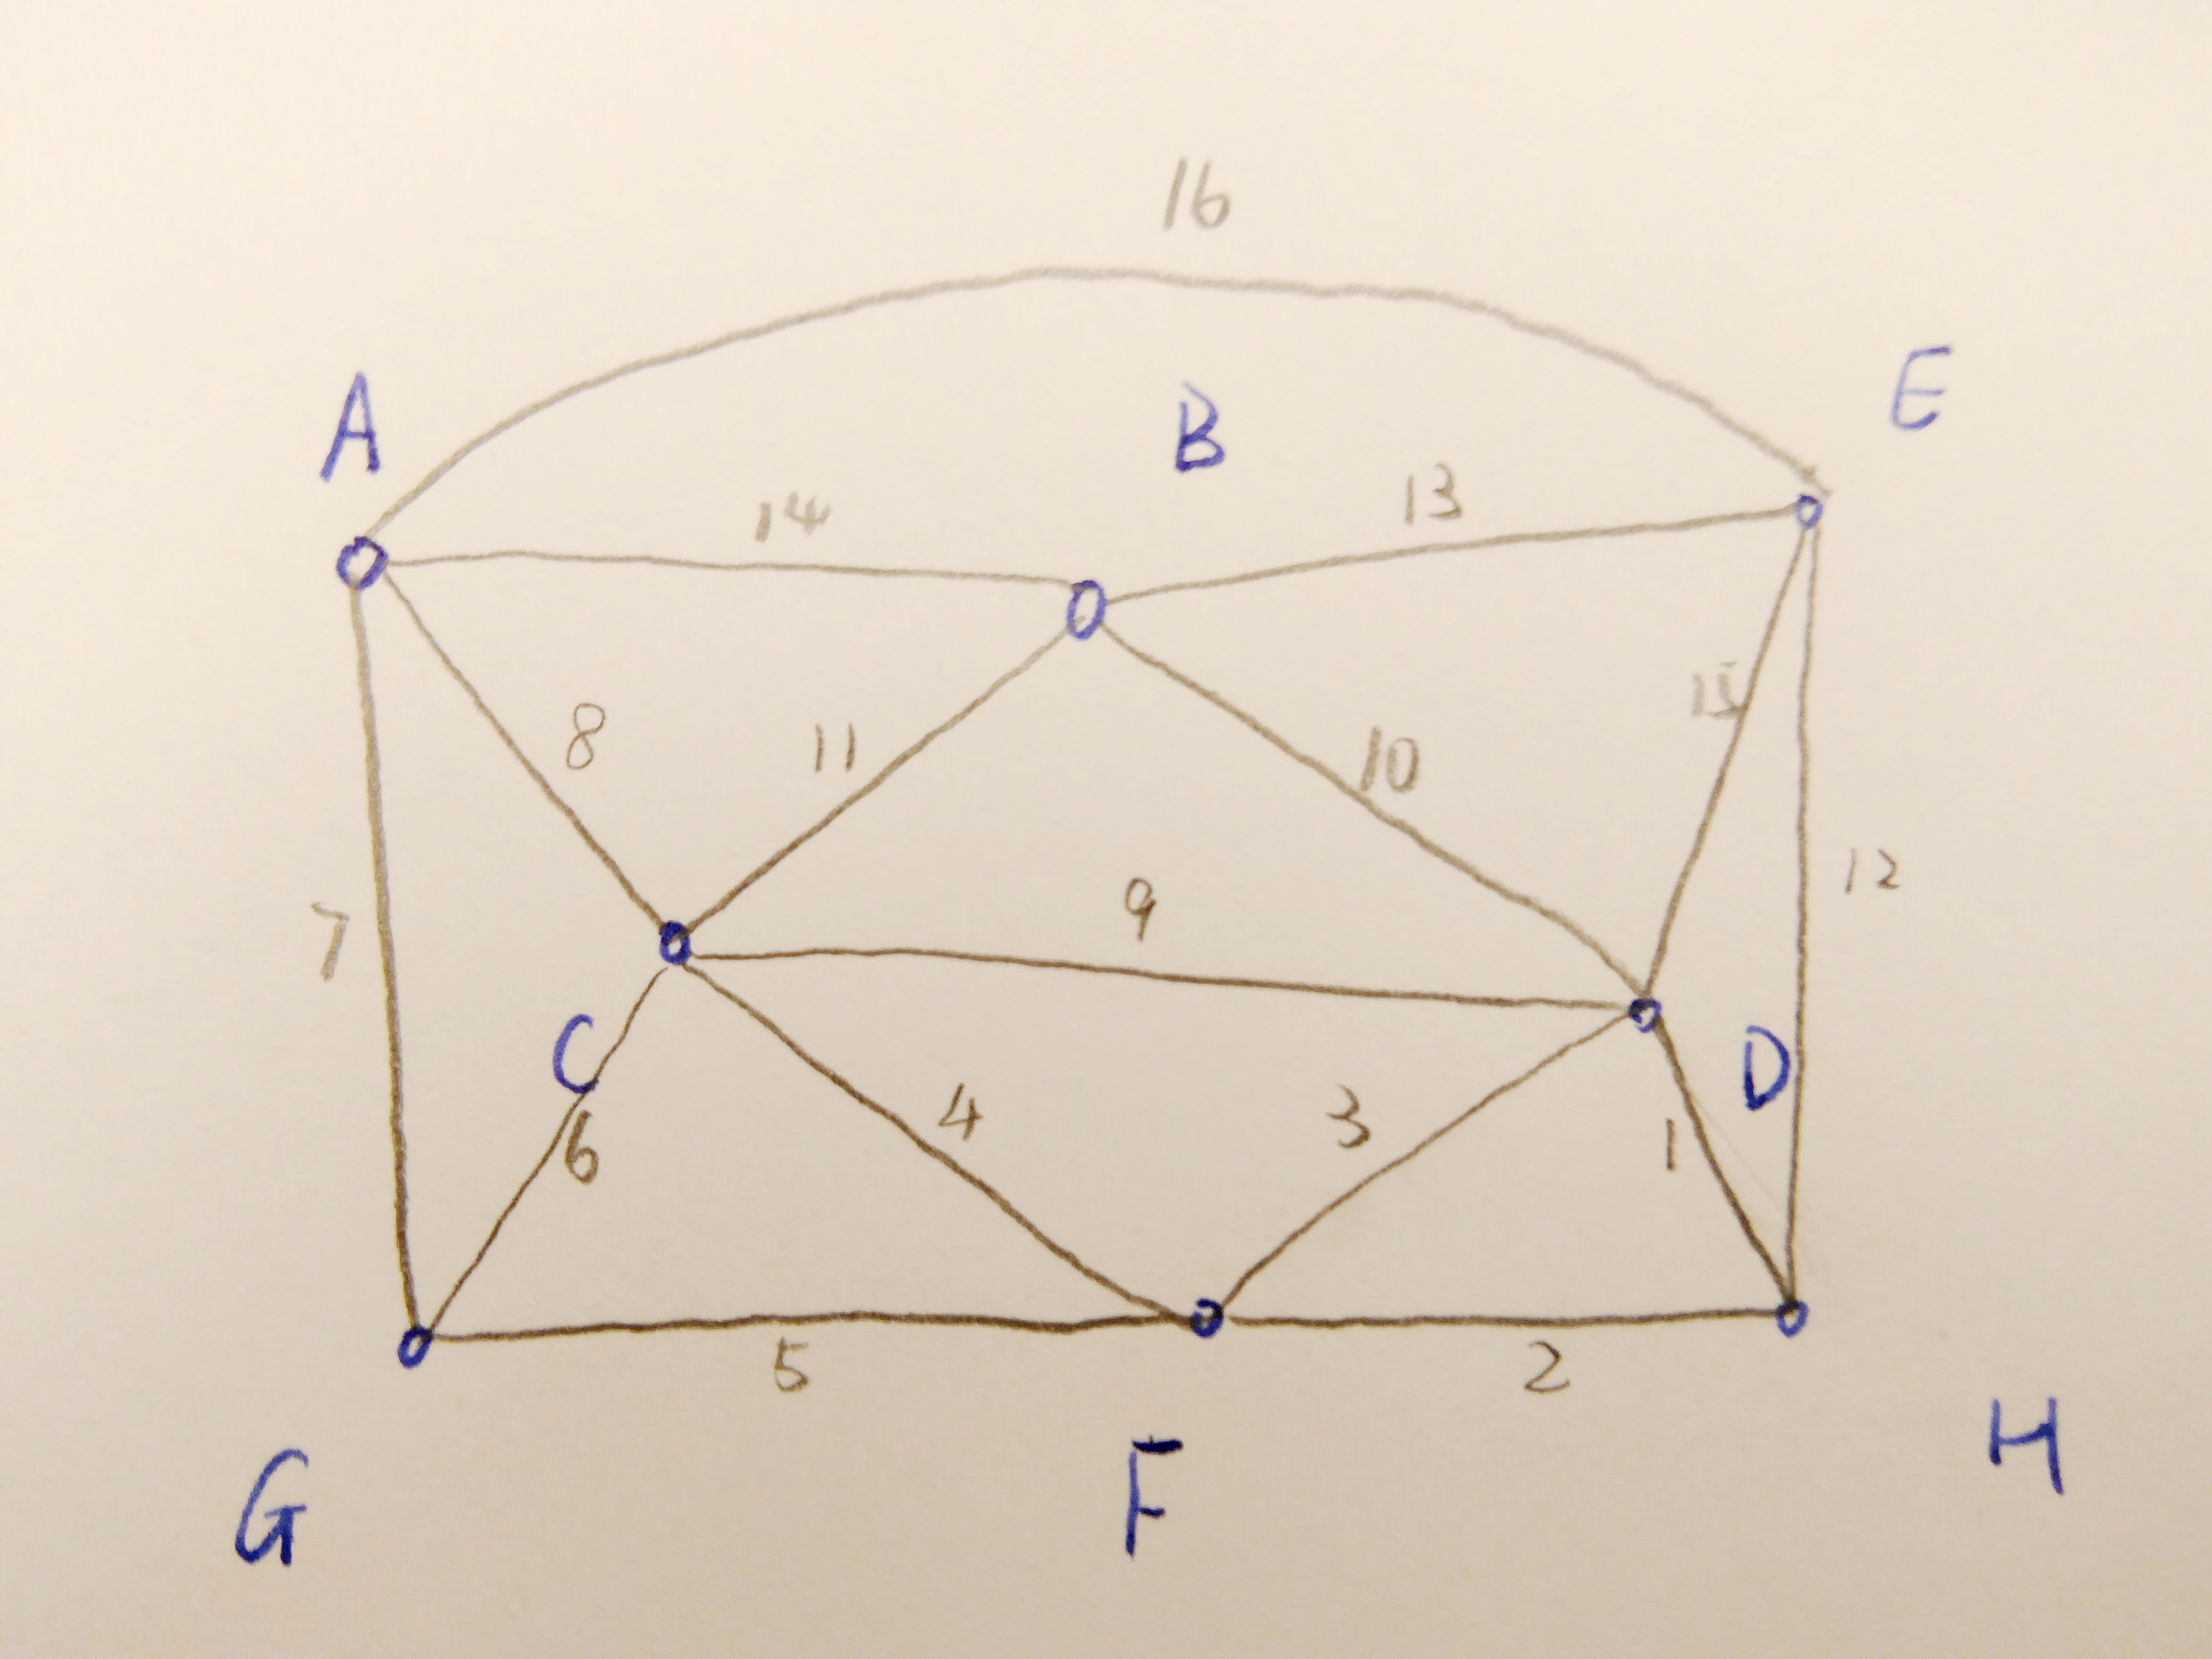
\includegraphics[width=0.85\linewidth]{Figure/1a1.jpg}
		\caption{Initial Figure}
		\label{fig:subfig1:a}
	\end{minipage}
	\begin{minipage}[t]{0.50\linewidth}
		\centering
		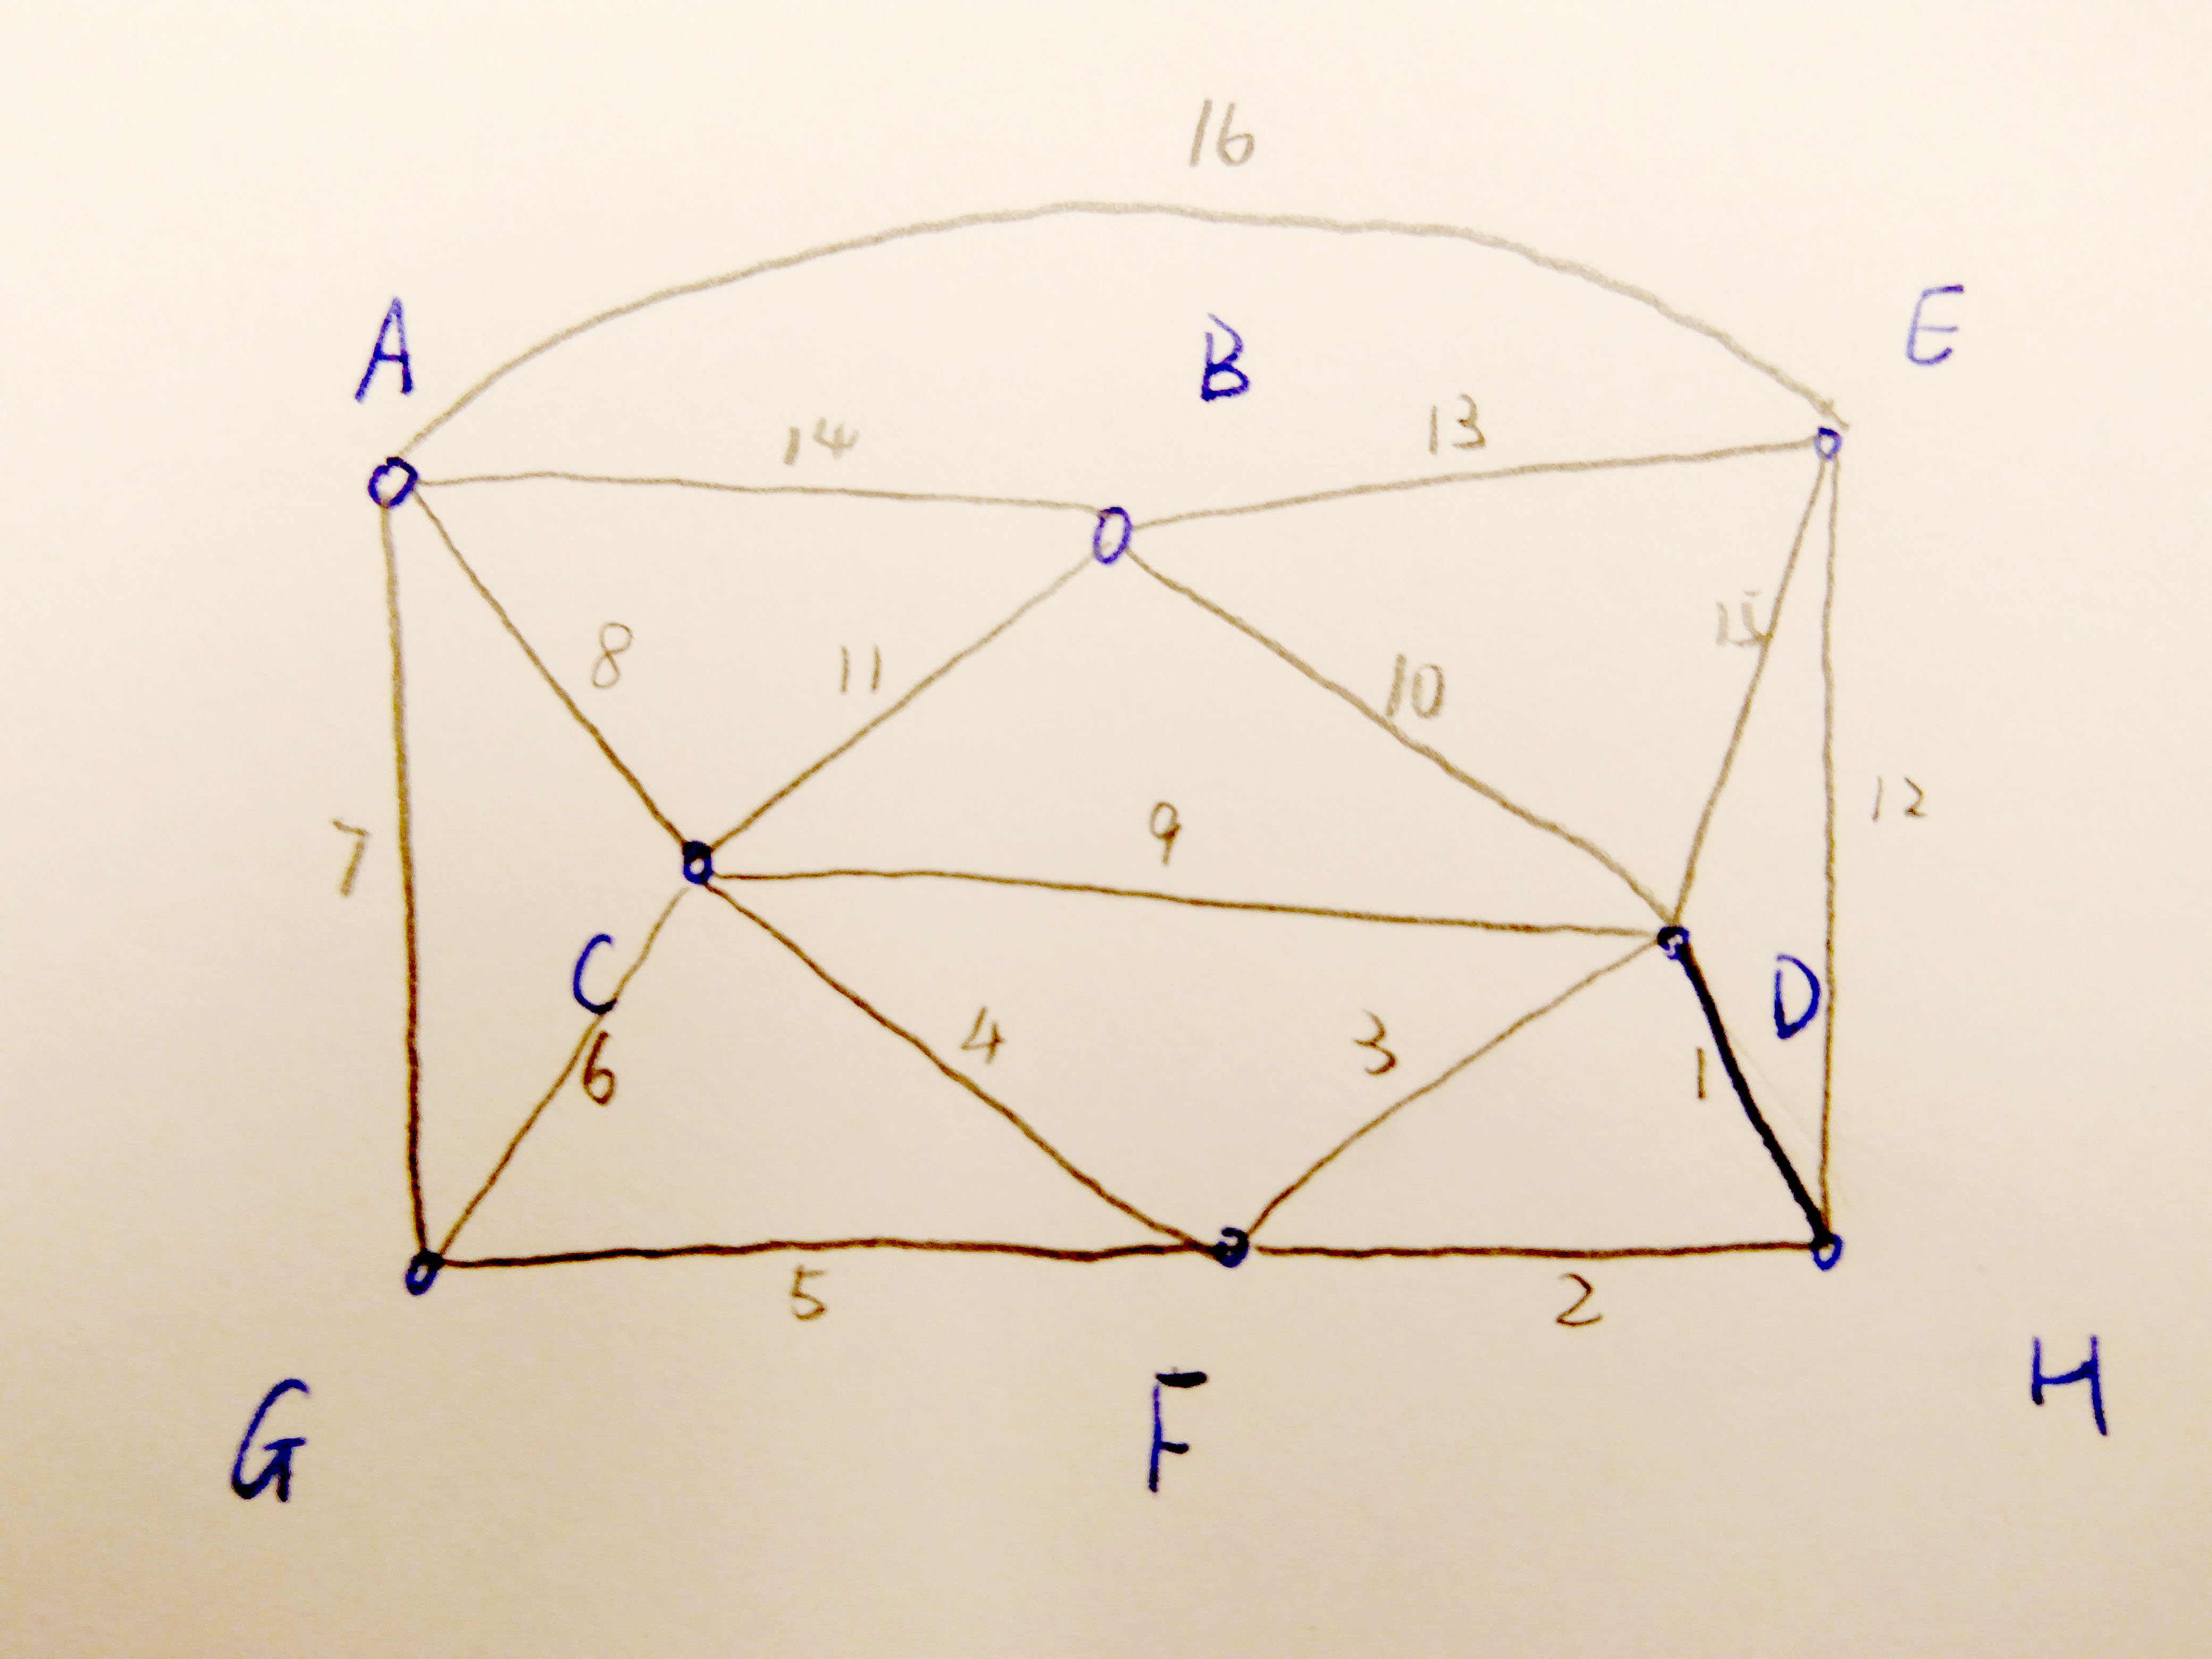
\includegraphics[width=0.85\linewidth]{Figure/1a2.jpg}
		\caption{Add $(D,H)$ to the tree}
		\label{fig:subfig1:b}
	\end{minipage}
\\
	\begin{minipage}[t]{0.50\linewidth}
		\centering
		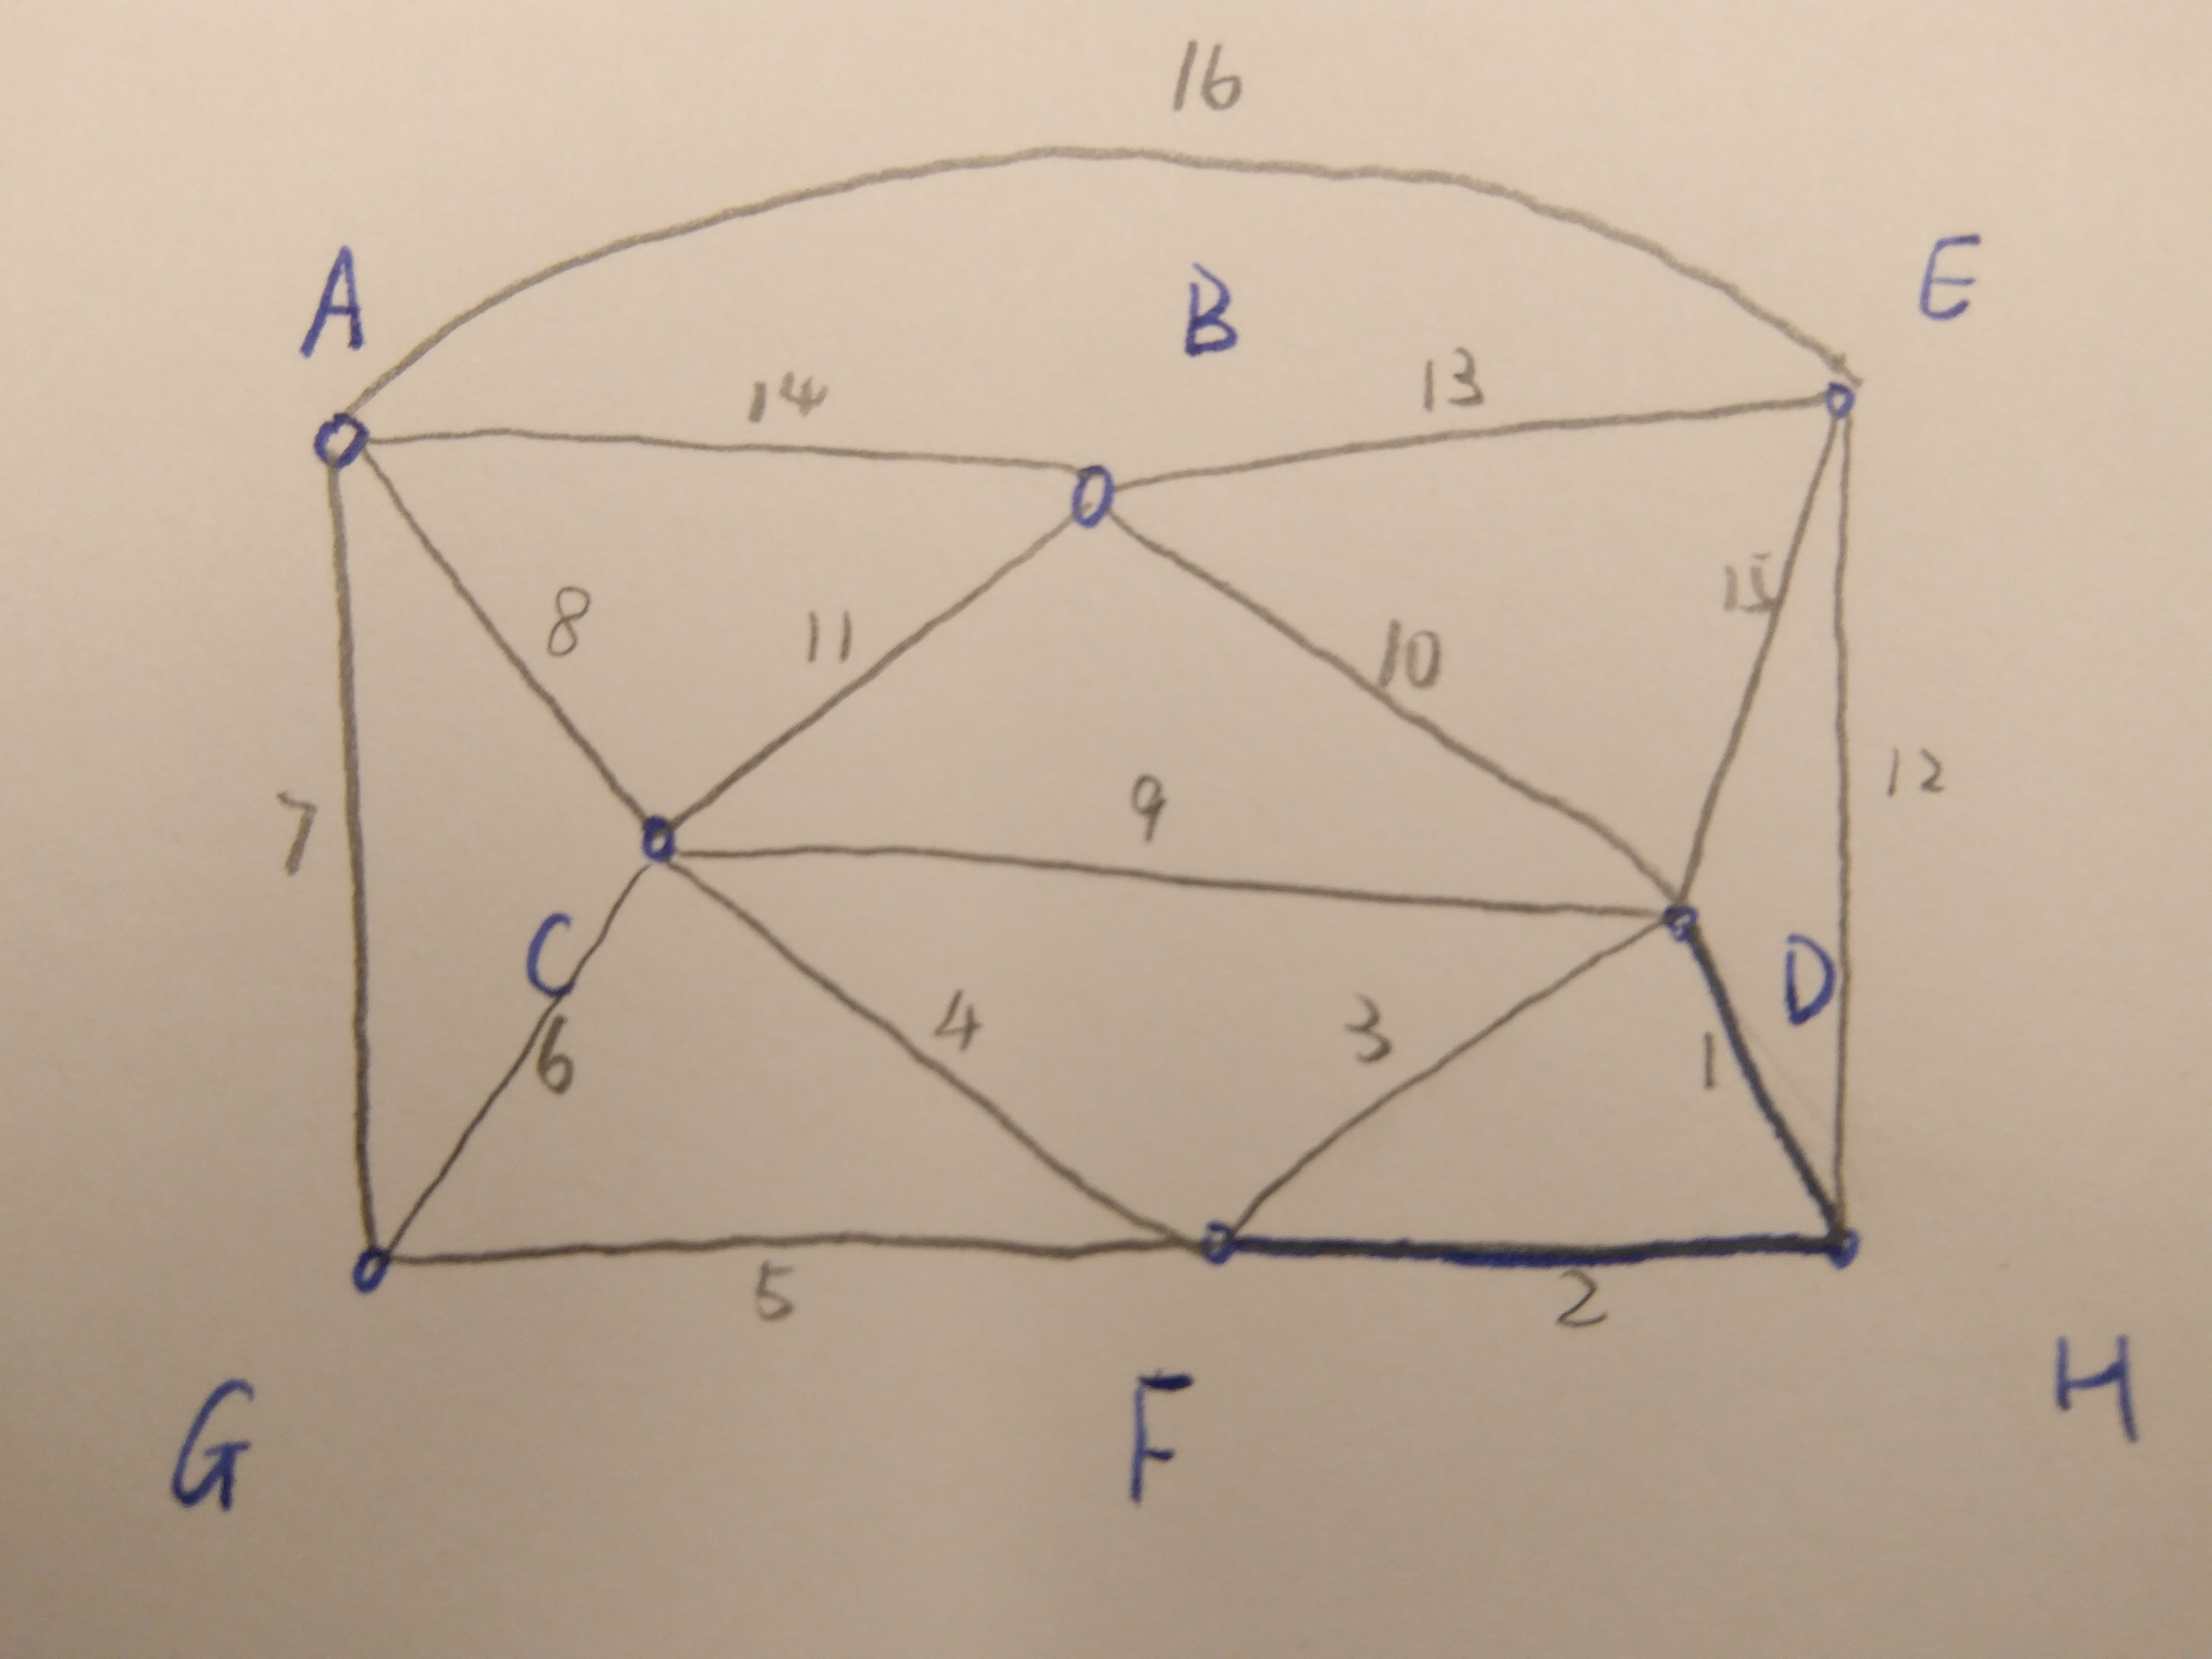
\includegraphics[width=0.85\linewidth]{Figure/1a3.jpg}
		\caption{Add $(F,H)$ to the tree}
		\label{fig:subfig1:c}
	\end{minipage}
	\begin{minipage}[t]{0.50\linewidth}
		\centering
		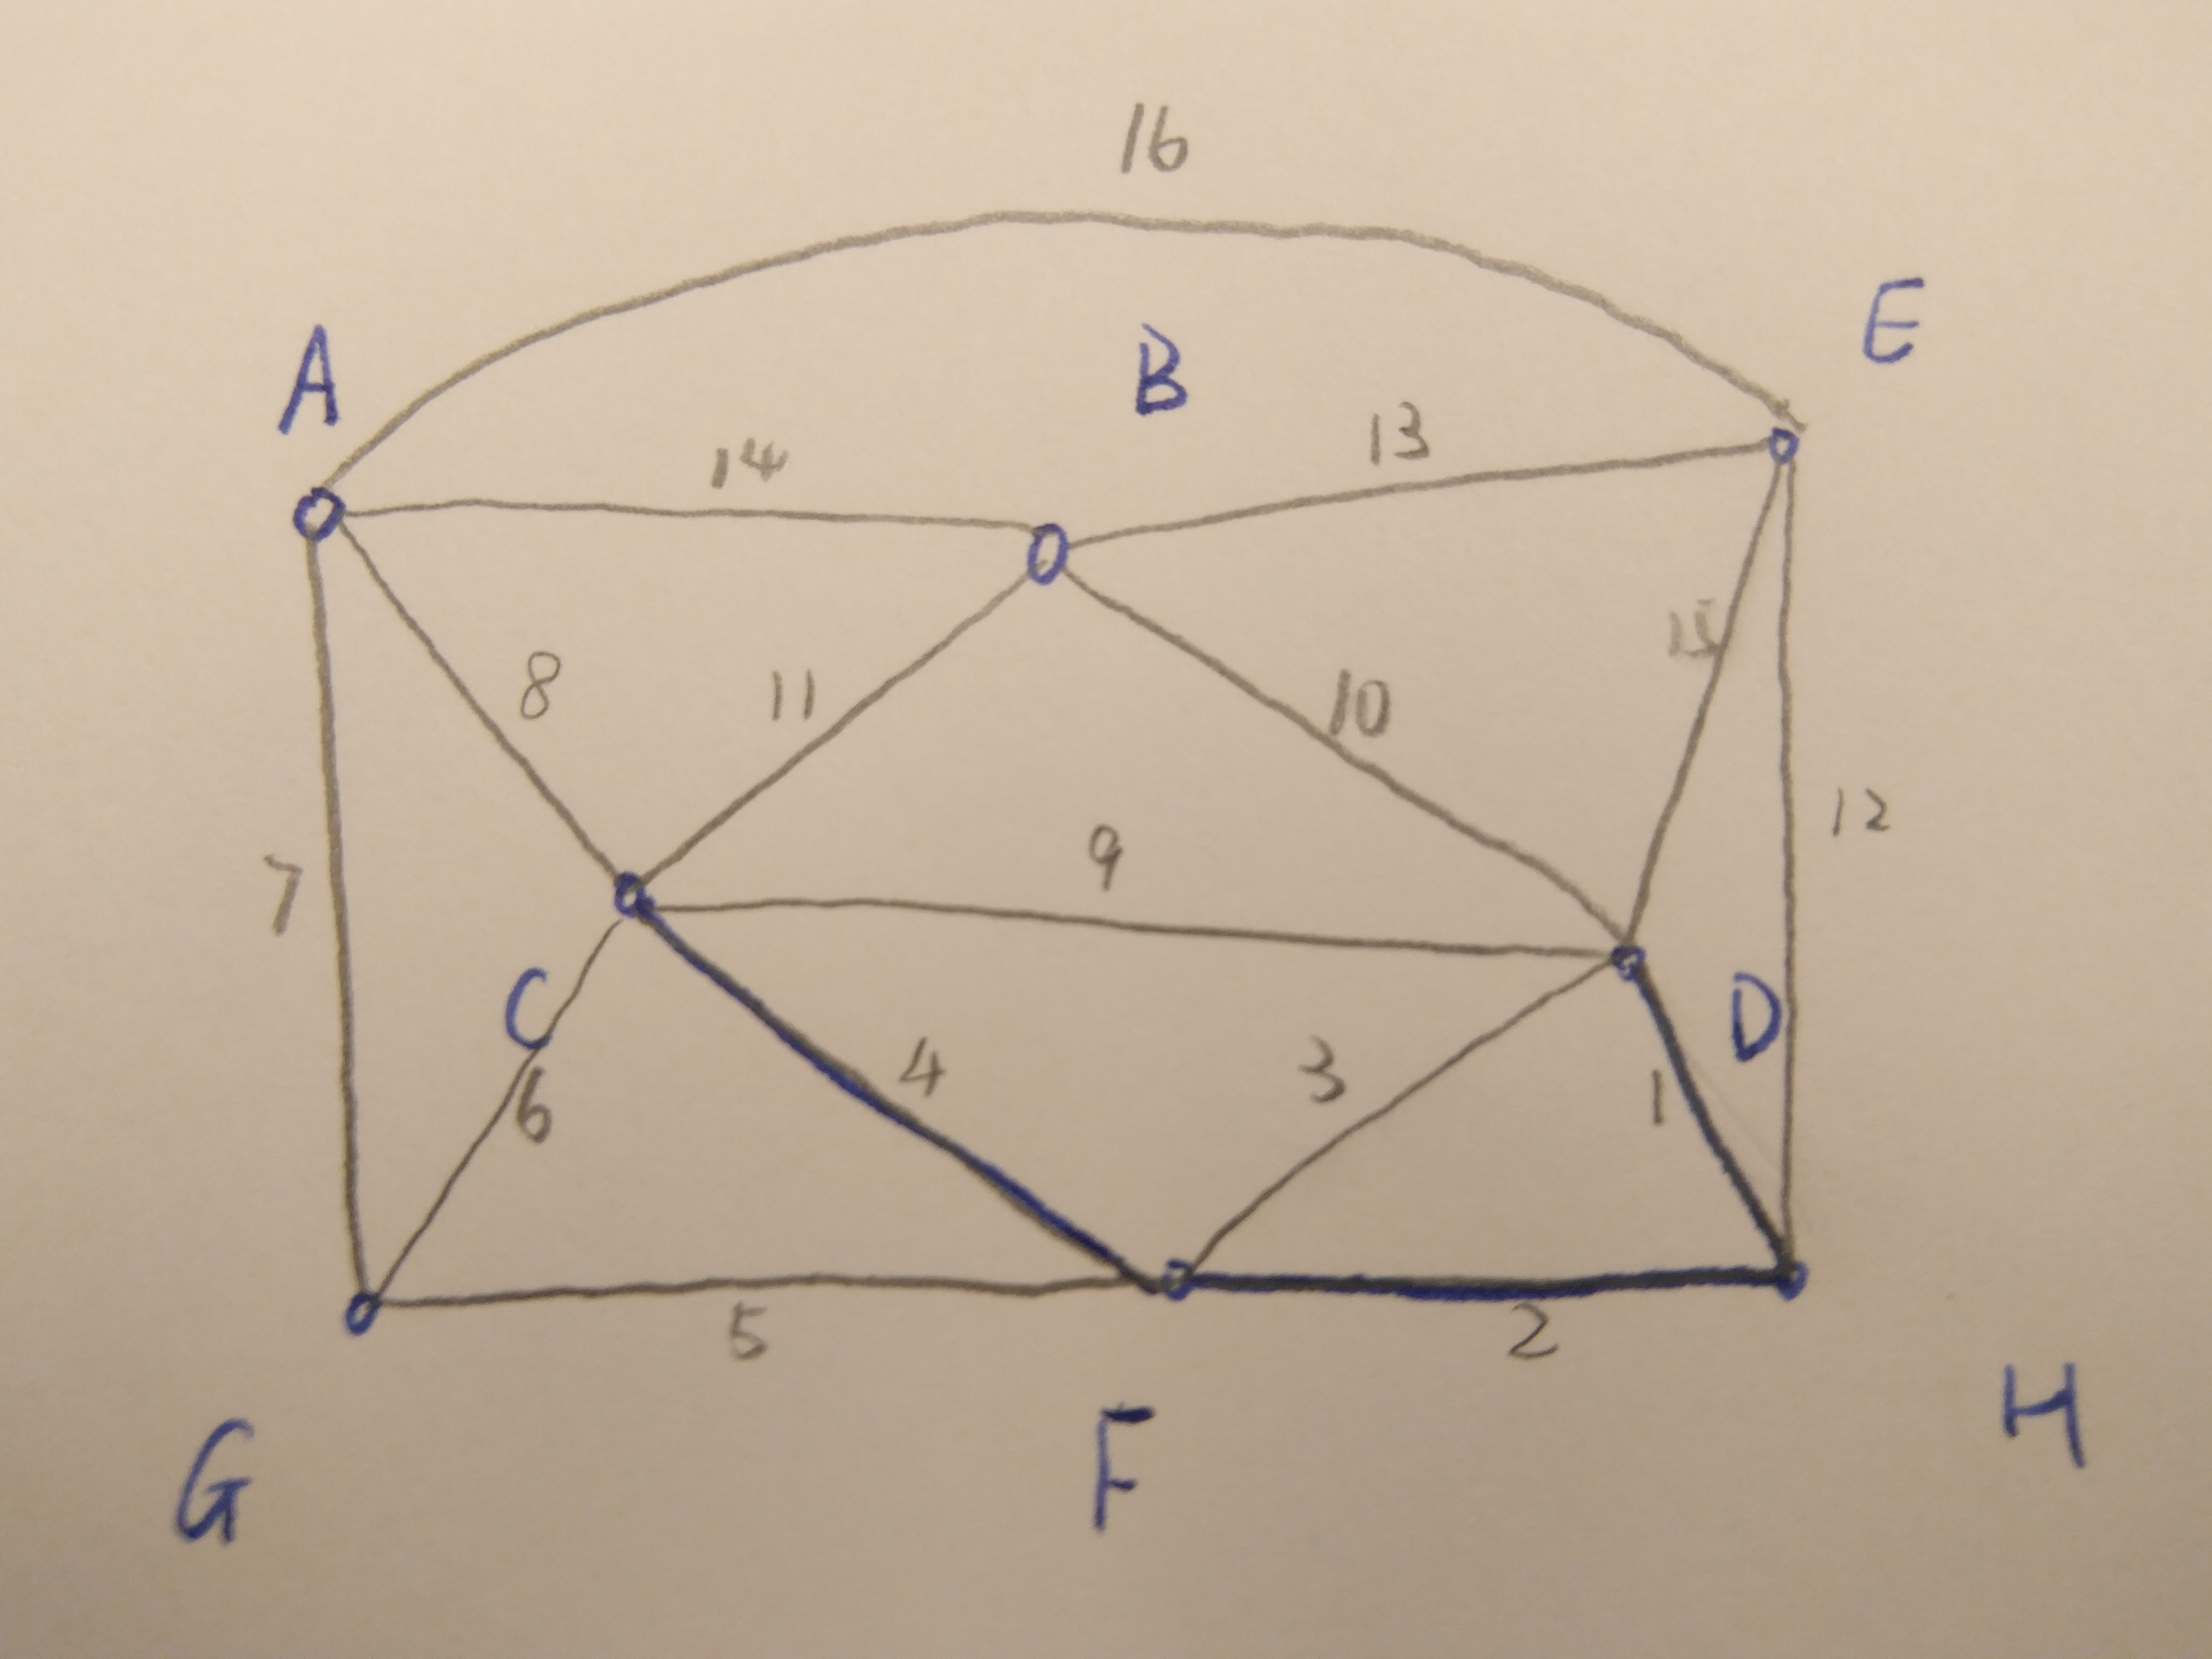
\includegraphics[width=0.85\linewidth]{Figure/1a4.jpg}
		\caption{Add $(C,F)$ to the tree}
		\label{fig:subfig1:d}
	\end{minipage}
\end{figure}
\begin{figure}[H]
	\begin{minipage}[t]{0.50\linewidth}
		\centering
		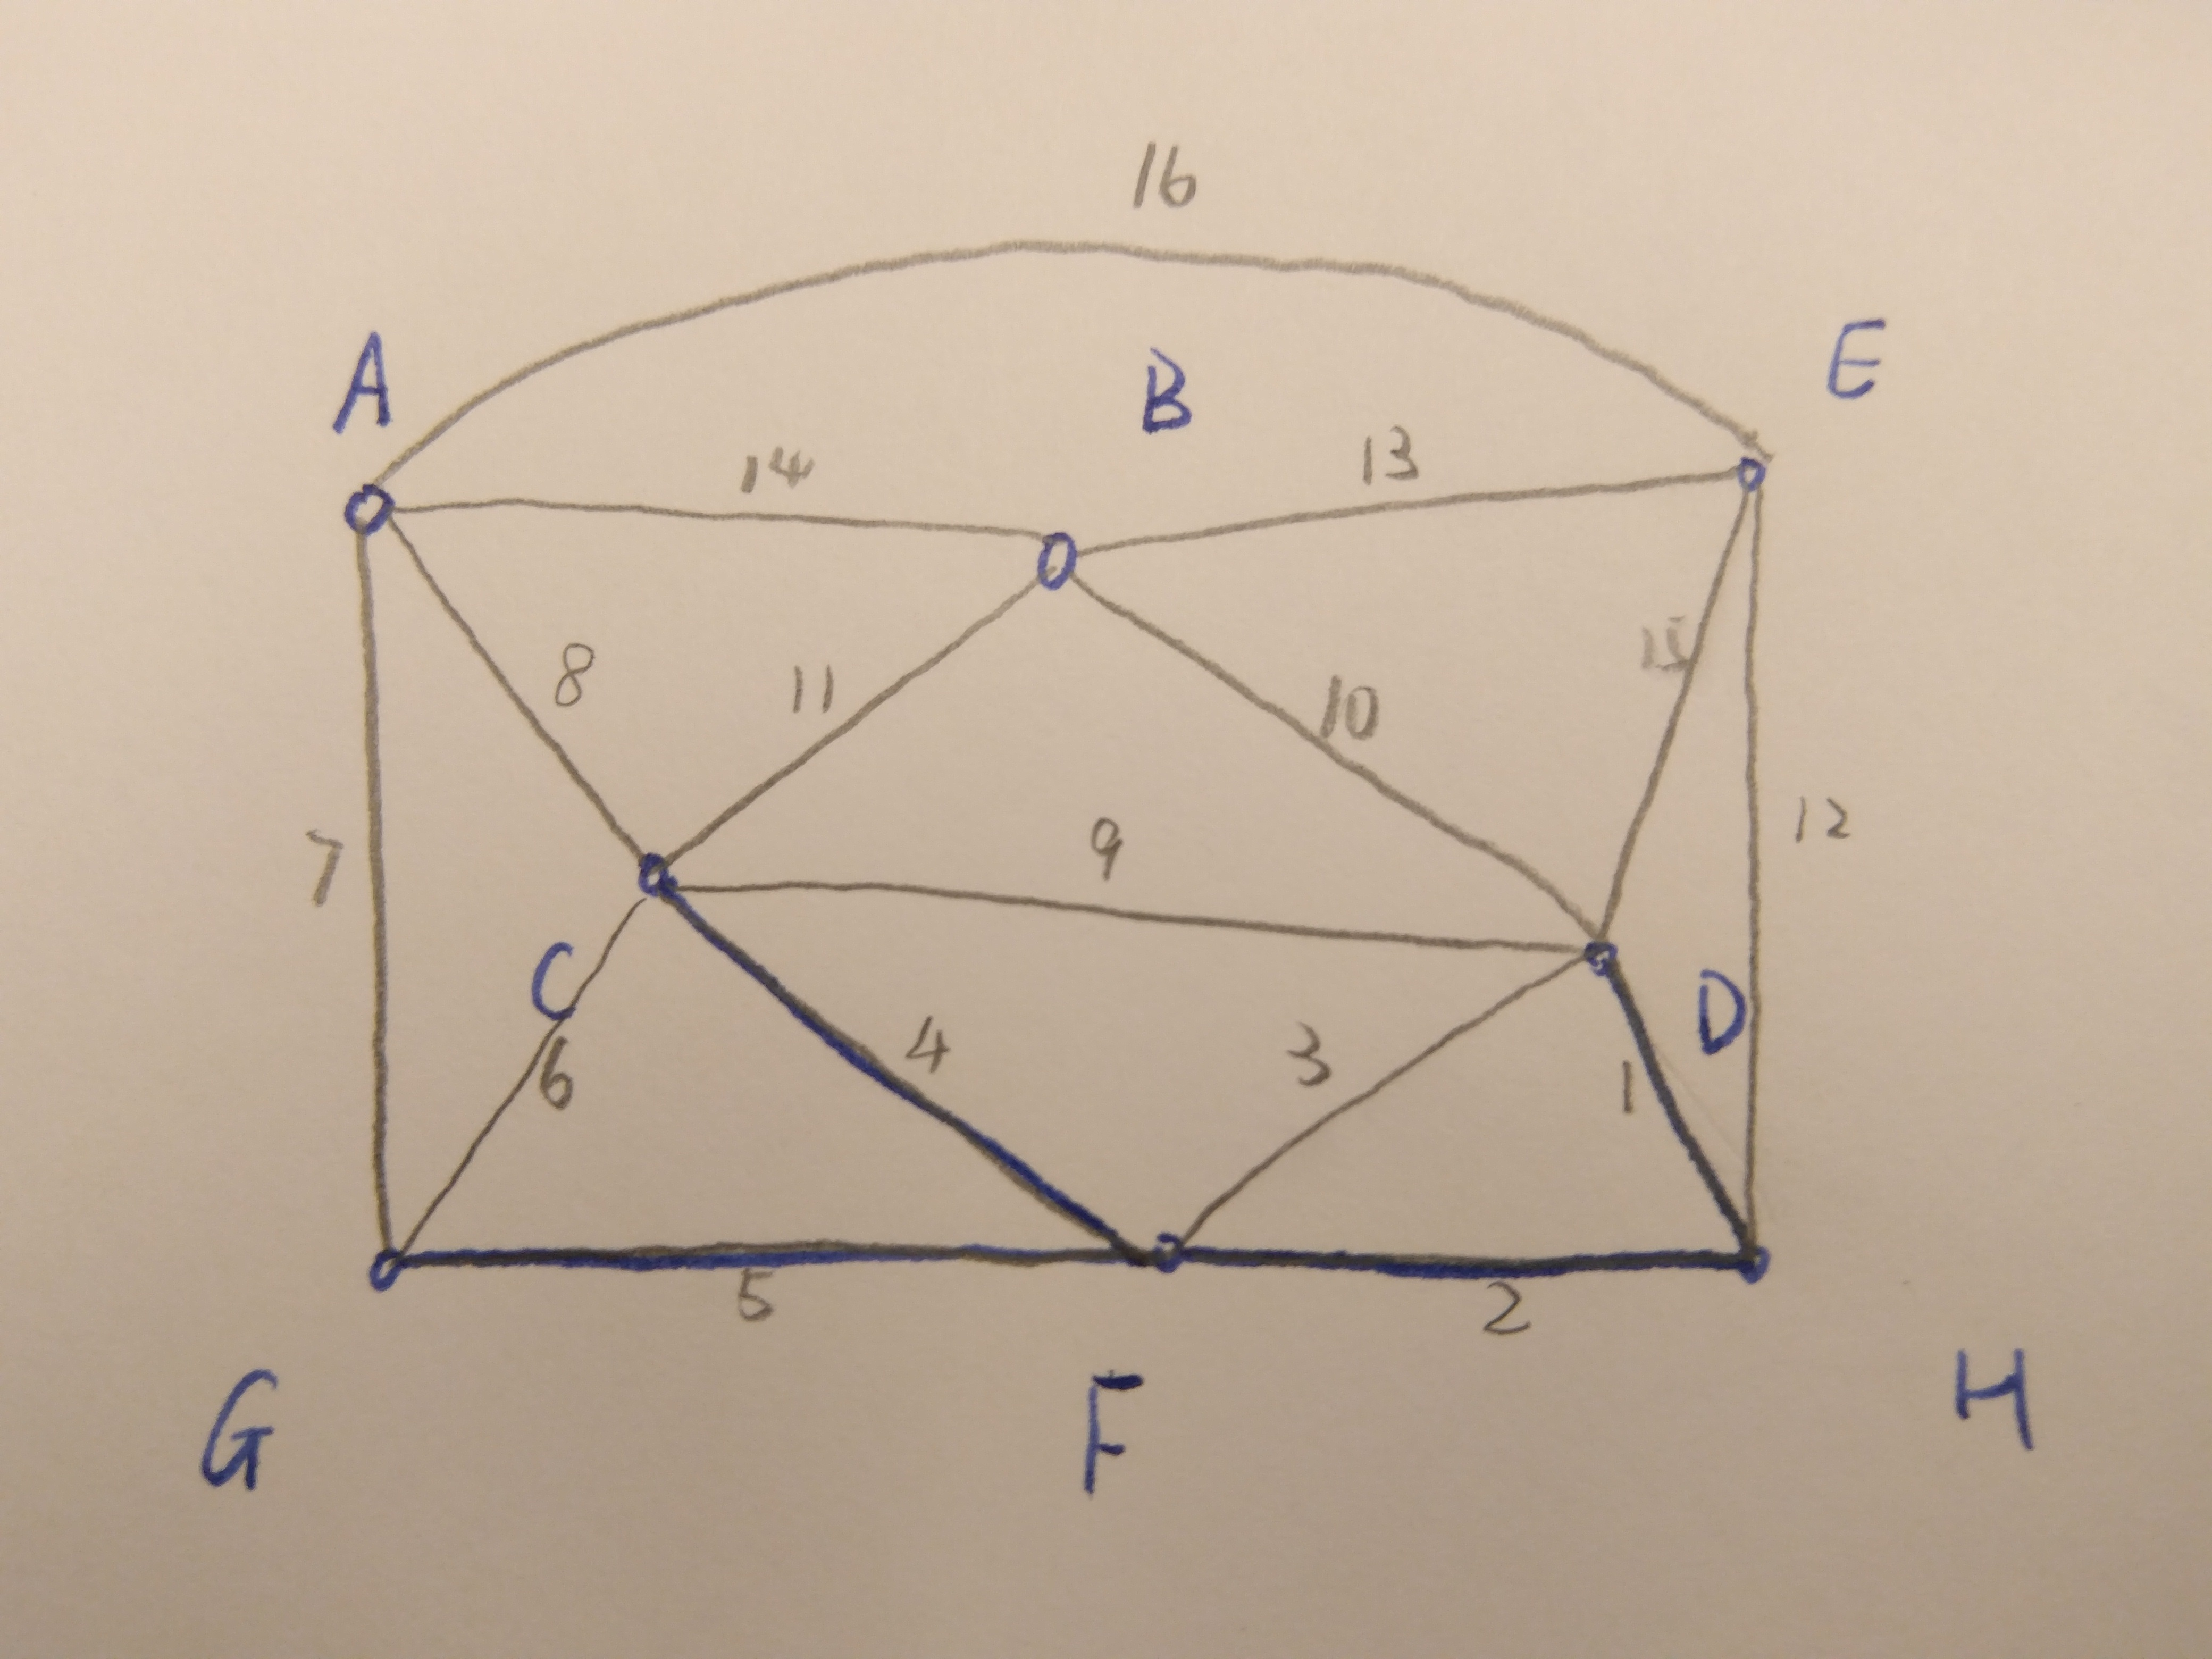
\includegraphics[width=0.85\linewidth]{Figure/1a5.jpg}
		\caption{Add $(G,H)$ to the tree}
		\label{fig:subfig1:e}
	\end{minipage}
	\begin{minipage}[t]{0.50\linewidth}
		\centering
		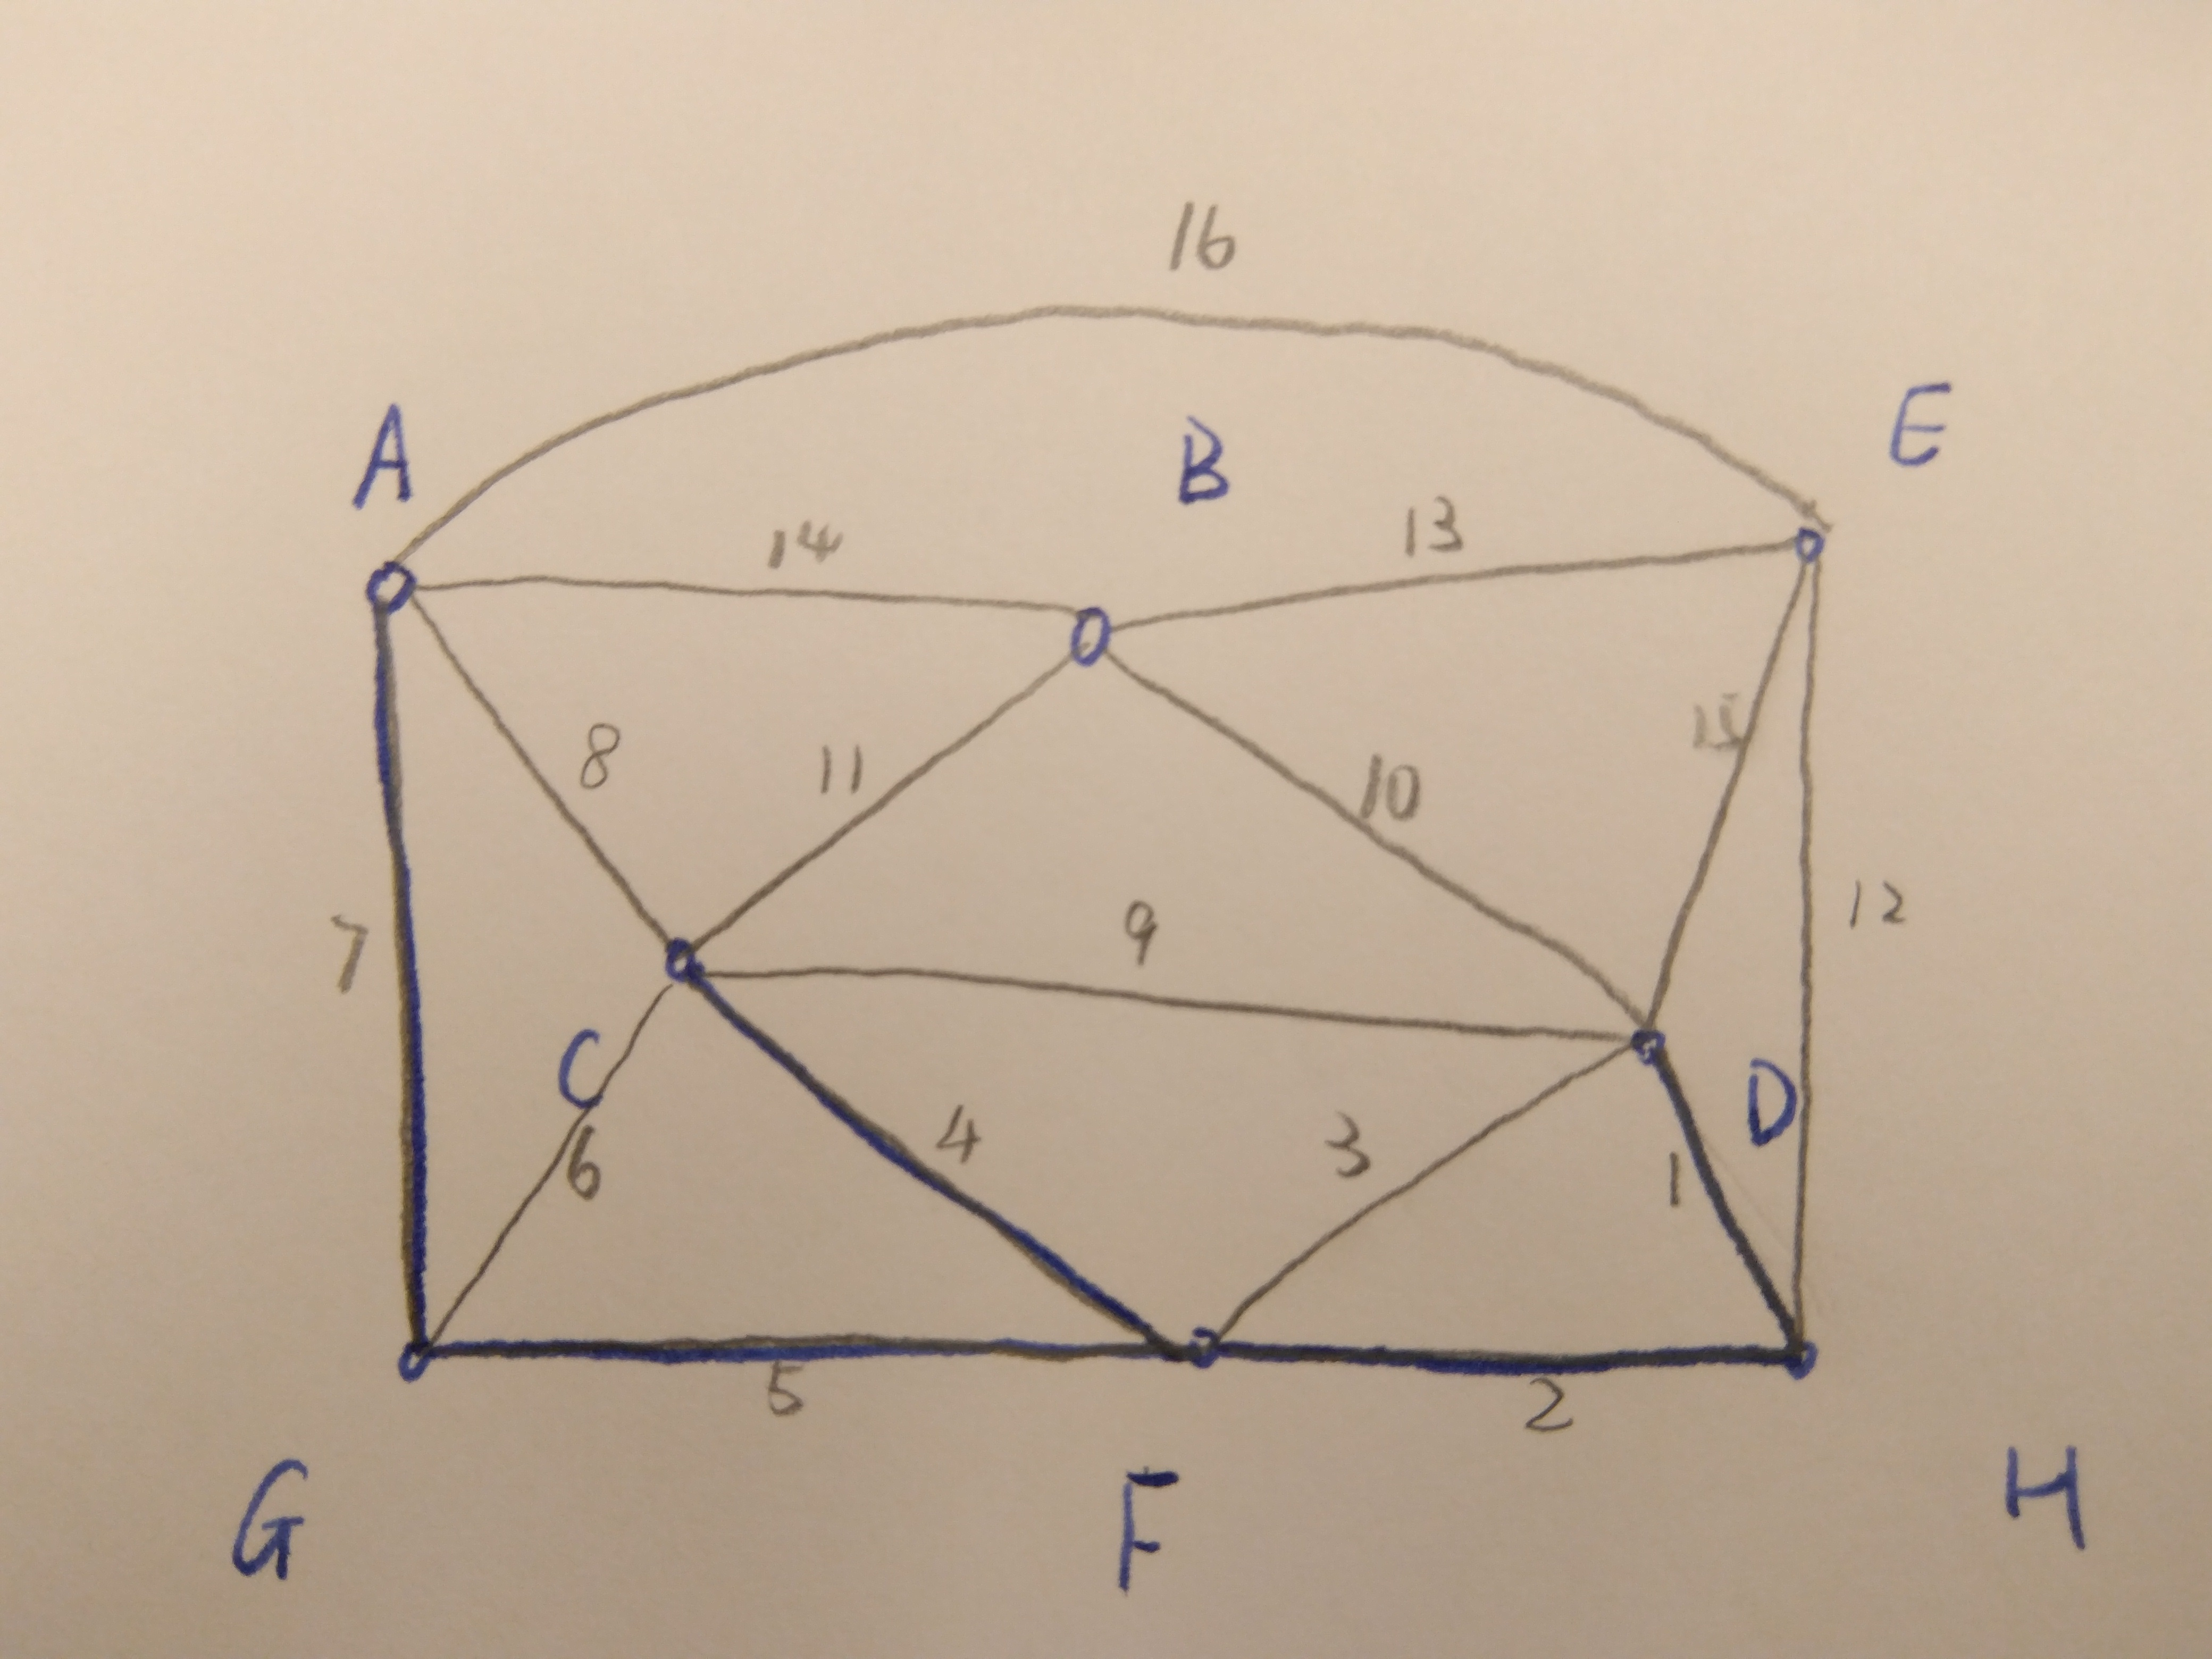
\includegraphics[width=0.85\linewidth]{Figure/1a6.jpg}
		\caption{Add $(A,G)$ to the tree}
		\label{fig:subfig1:f}
	\end{minipage}
\\
	\begin{minipage}[t]{0.50\linewidth}
		\centering
		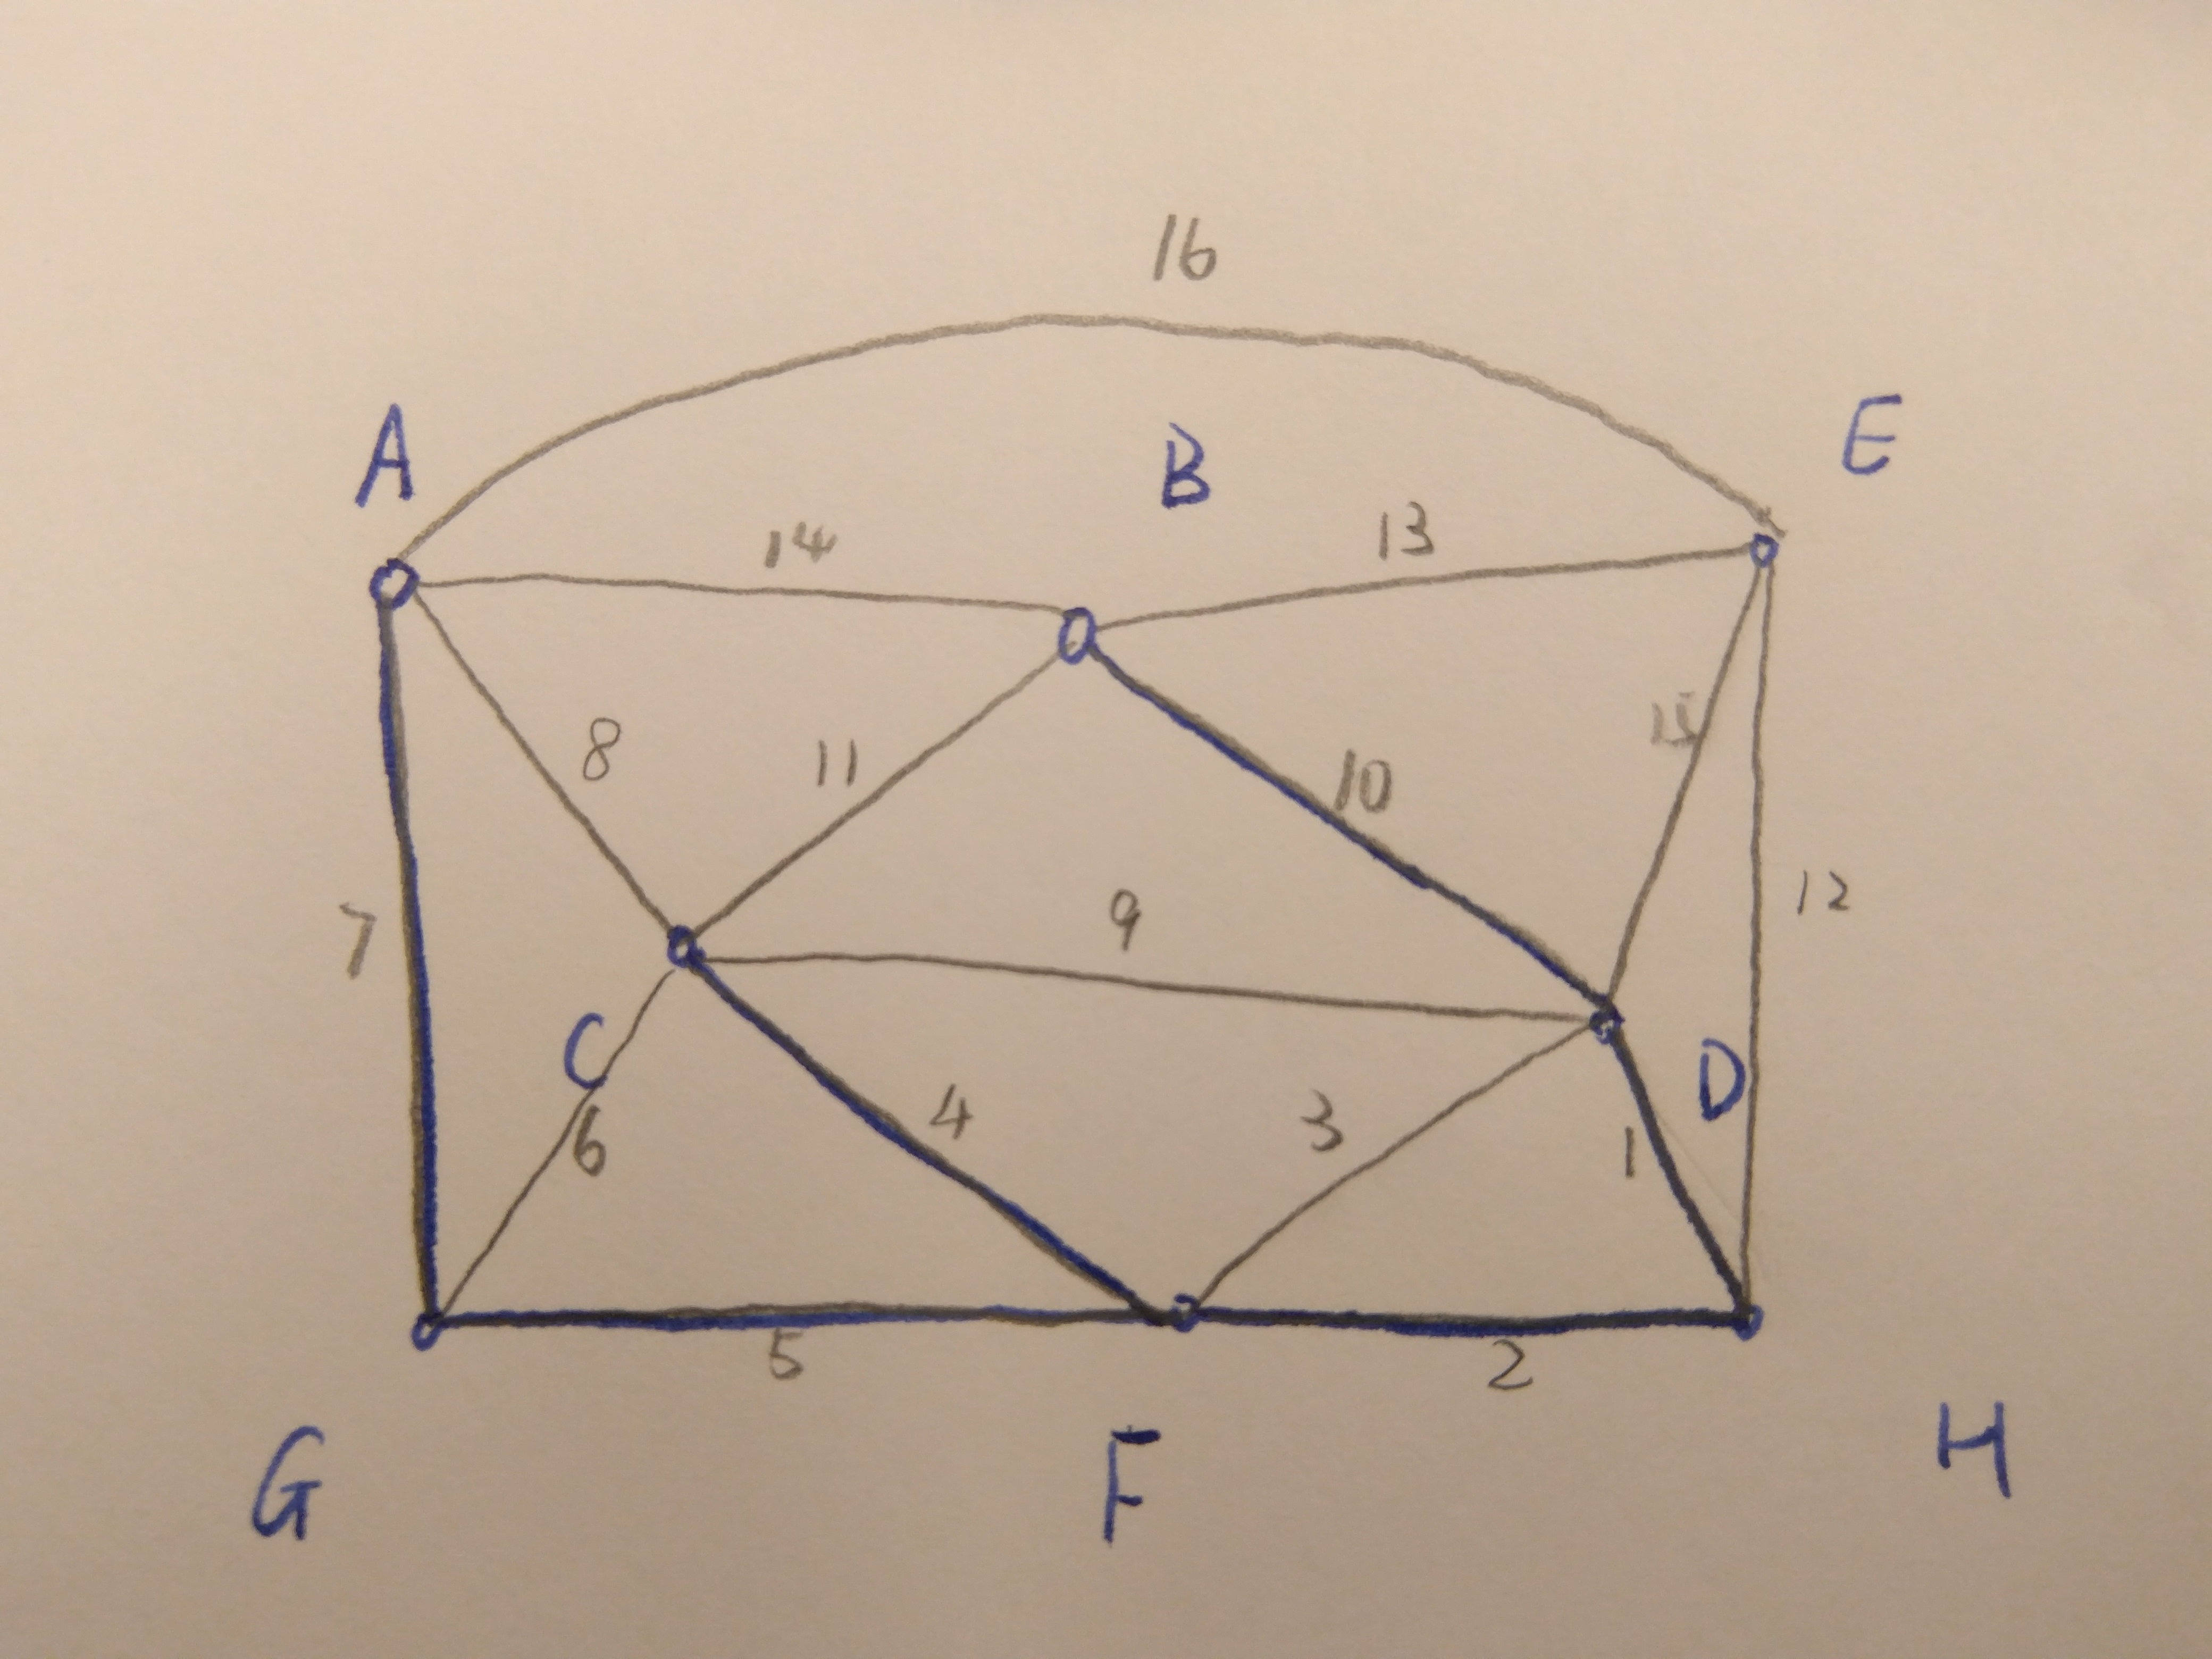
\includegraphics[width=0.85\linewidth]{Figure/1a7.jpg}
		\caption{Add $(B,D)$ to the tree}
		\label{fig:subfig1:g}
	\end{minipage}
	\begin{minipage}[t]{0.50\linewidth}
		\centering
		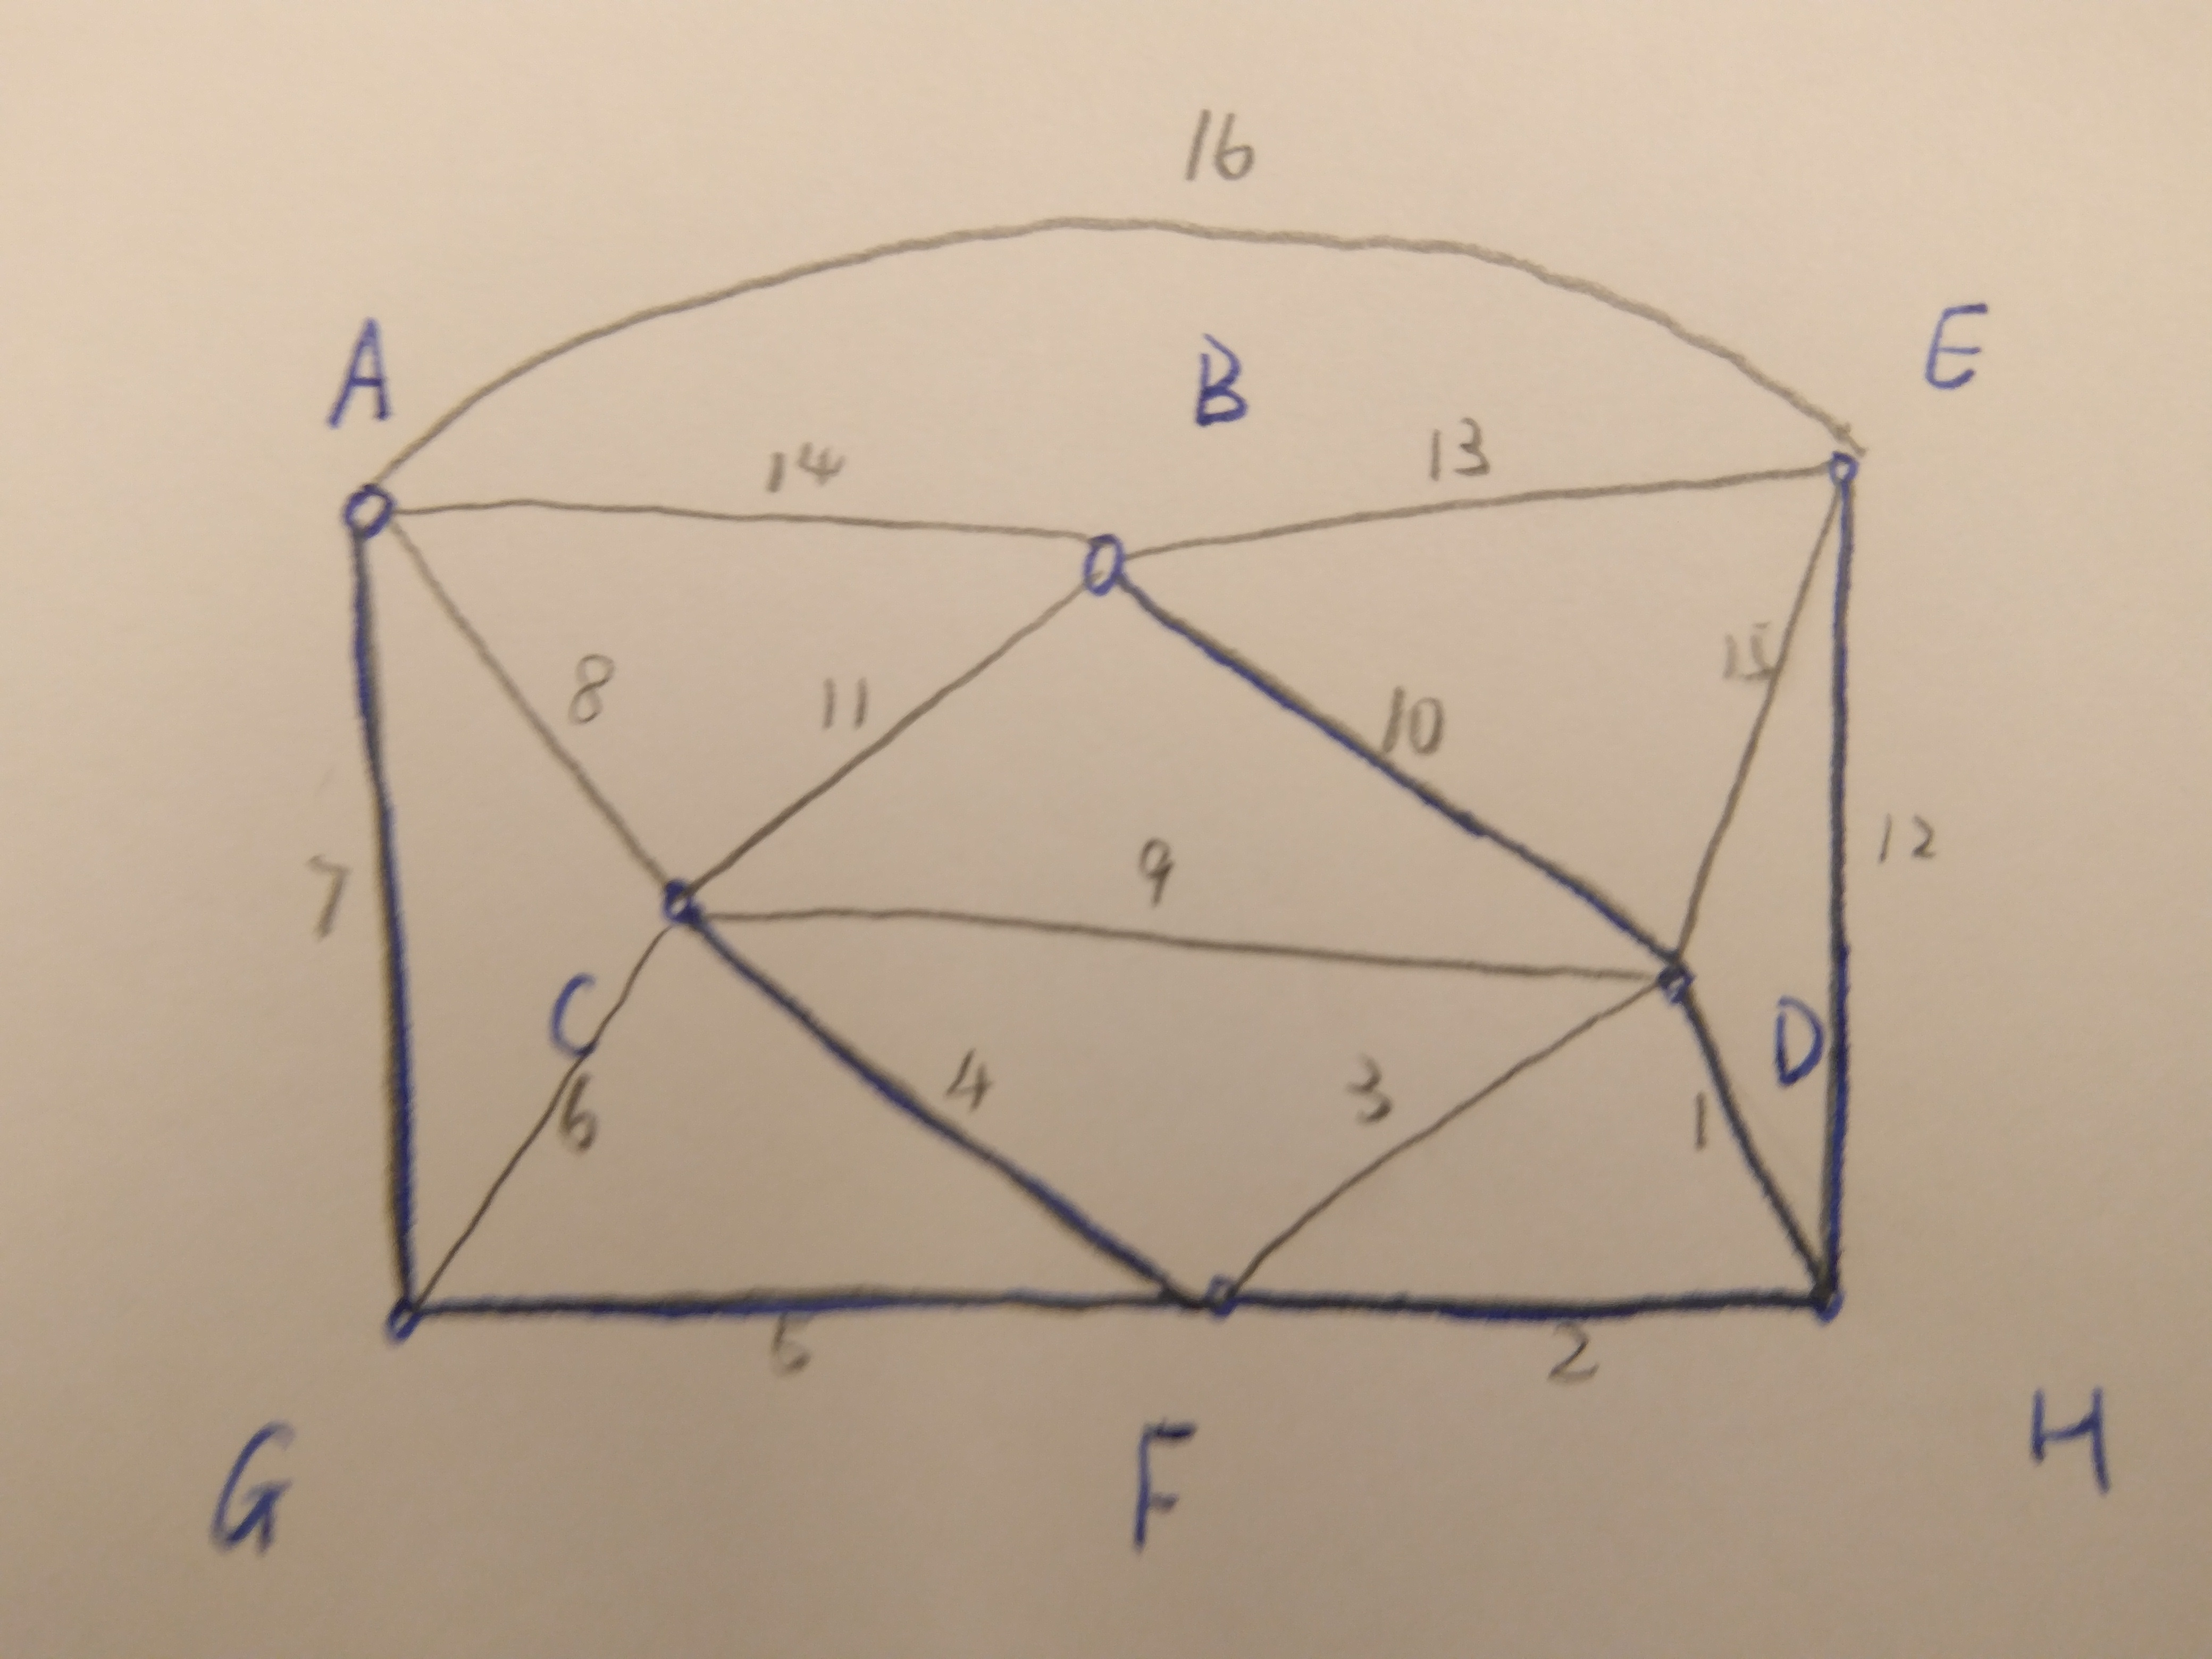
\includegraphics[width=0.85\linewidth]{Figure/1a8.jpg}
		\caption{Add $(E,H)$ to the tree}
		\label{fig:subfig1:h}
	\end{minipage}
\end{figure}
\subsection{R-18.3}
Give an example of a graph $G$ with at least $10$ vertices such that the greedy 2-approximation algorithm for VERTEX-COVER given above is guaranteed to produce a suboptimal vertex cover.

\noindent \textbf{\emph{Answer}}:
The initial graph is shown in Fig.\ref{fig:subfig2:a}, which contains $10$ vertice, and the process of 2-approximation algorithm is shown in Fig\ref{fig:subfig2:a} through \ref{fig:subfig2:d}. As we can see in Fig.\ref{fig:subfig2:d}, to cover edge$(v_3,v_4)$, we must either add $v_3$ or $v_4$ to the set $C$, which must at least contain $7$ elements. However, we can simply conclude from the initial graph that set $C=\{v_2,v_3,v_5,v_6,v_7,v_9\}$ can be a better VERTEX COVER for the initial graph which have $6$ vertices. Such example proved that this greedy approximation algorithm will produce a suboptimal result.
\begin{figure}[H]
	\begin{minipage}[t]{0.50\linewidth}
		\centering
		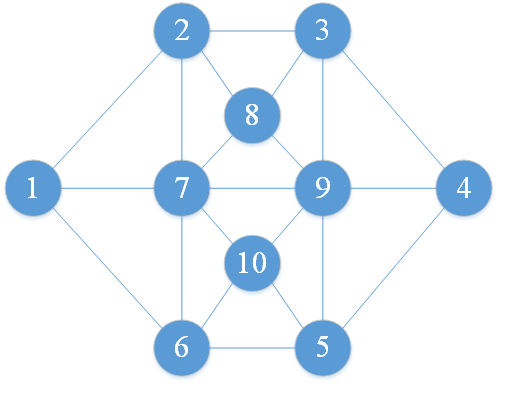
\includegraphics[width=0.75\linewidth]{Figure/1b1.png}
		\caption{Initial Graph}
		\label{fig:subfig2:a}
	\end{minipage}
	\begin{minipage}[t]{0.50\linewidth}
		\centering
		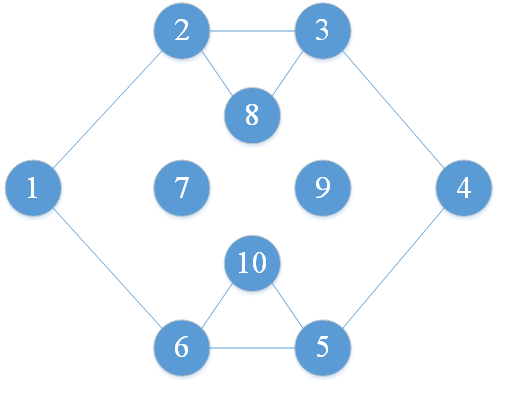
\includegraphics[width=0.75\linewidth]{Figure/1b2.png}
		\caption{Add $v_7$ and $v_9$ to the $C$}
		\label{fig:subfig2:b}
	\end{minipage}
	\\
		\begin{minipage}[t]{0.50\linewidth}
		\centering
		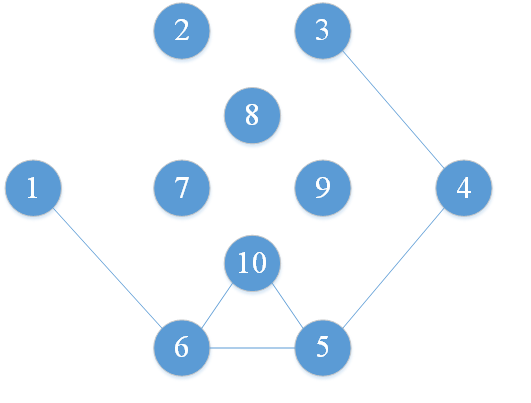
\includegraphics[width=0.75\linewidth]{Figure/1b3.png}
		\caption{Add $v_2$ and $v_8$ to the $C$}
		\label{fig:subfig2:c}
	\end{minipage}
	\begin{minipage}[t]{0.50\linewidth}
		\centering
		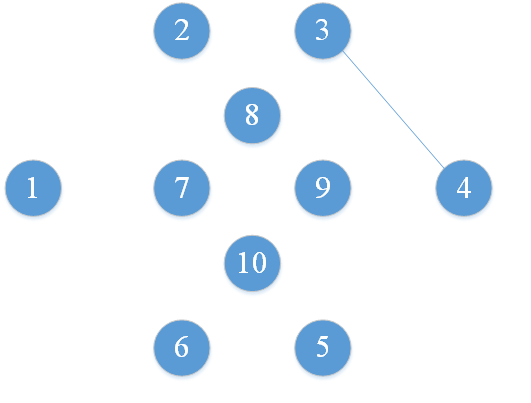
\includegraphics[width=0.75\linewidth]{Figure/1b4.png}
		\caption{Add $v_6$ and $v_5$ to the $C$}
		\label{fig:subfig2:d}
	\end{minipage}
\end{figure}
\section{Dijkstra Revisited}
There is an alternative way of implementing Dijkstra’s algorithm that avoids use of the locator pattern but increases the space used for the priority queue, $Q$, from $O(n)$ to $O(m)$ for a weighted graph, $G$, with $n$ vertices and $m$ edges. The main idea of this approach is simply to insert a new key-value pair, $(D[v], v)$, each time the $D[v]$ value for a vertex, $v$, changes, without ever removing the old key-value pair for $v$. This approach still works, even with multiple copies of each vertex being stored in $Q$, since the first copy of a vertex that is removed from $Q$ is the copy with the smallest key. Describe the other changes that would be needed to the description of Dijsktra’s algorithm for this approach to work. Also, what is the running time of Dijkstra’s algorithm in this approach if we implement the priority queue, $Q$, with a heap?

\noindent \textbf{\emph{Answer}}: The algorithm is shown as follows:
\begin{algorithmic}
	\State \textbf{Algorithm} Dijkstra($G,v$)
	\State \textbf{Input}: A connected graph $G$, a root vertex $v$
	\State \textbf{Output}: the list of shortest distance from the root vertex to all the other vertices.
	\State $Q\gets$ an empty priority queue that stores $(w,v)$ pair
	\State $P\gets$ an empty list
	\State $visited \gets v$ \Comment a list that records visited vertices.
	\State $P.push(v)$
	\While{$P$ is not $NULL$}
		\State $c\gets P.popMinimum(Q,visited)$\Comment Like a BFS
		\State $visited.push(c)$
		\For{$n$ in $neighbor(c)$}
			\State $P.push(n)$
			\If {not $Q.contain(n)$ or $weight(c,n)+Q.getWeight(c)<Q.getWeight(n)$}
				\State $Q.push((weight(c,n)+Q.getWeight(c)),n)$
			\EndIf
		\EndFor
	\EndWhile
	\State $D\gets $an empty list
	\For {$i$ in $V$}\Comment $V$ is the set of all the vertices in $G$
		\State $D[i]\gets Q.getWeight(v)$
	\EndFor
\end{algorithmic}

Note in the algorithm, $Q.getWeight(n)$ returns the weight of vertice $n$ in queue $Q$. $weight(n,c)$ returns the weight of edge between $n$ and $c$, $Q.contain(n)$ returns whether there is $n$ in the queue $Q$. The $P.popMinimum()$ returns the element in $P$ which has the smallest distance from the starting point $v$ as is recorded in $Q$, and the returning element is not visited as is recorded in $visited$.

In this algorithm, it will go over a process like BFS, which costs $O(|E|+|V|)$ time, and the popping method of $Q$ also costs $O(\log n)$ time when $Q$ has a size of $n$. Thus the total runtime would be $O(|E|+|V|\log |V|)$.
\section{The Struggle of Commuter Students}
Given an undirected weighted graph $G=(V,E)$ with non-negative edge weights, and two vertices $s,t\in V$, let $G'$ be $G$, but where every edge has its weight increased by $1$. Prove that $G$ and $G'$ have the same set of shortest paths from $s$ to $t$, or provide a counterexample.

\noindent \textbf{\emph{Answer}}: $G$ and $G'$ may not have the same set of shortest paths from $s$  to $t$. As is shown in Fig.\ref{fig:3}, the path $s\rightarrow a\rightarrow c\rightarrow d\rightarrow t$ has the least cost which is $11$. However, when all the edges have their weight increased by $1$, the former path would cost $15$ while another path $s\rightarrow b\rightarrow t$ would cost $14$. Thus this case becomes a counterexample.
\begin{figure}[H]
	\centering
	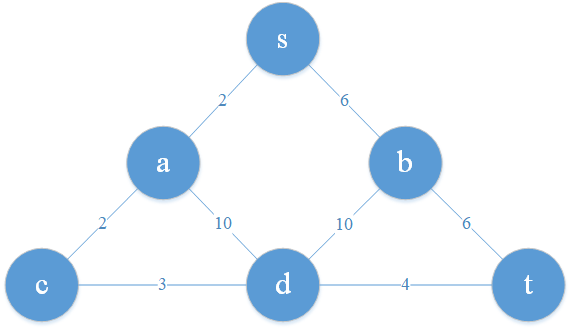
\includegraphics[width=0.60\linewidth]{Figure/3.png}
	\caption{A counterexample, number on an edge is the edge's cost}
	\label{fig:3}
\end{figure}
\section{Unique Bonsai}
Suppose $G$ is an undirected, connected, weighted graph such that the edges in $G$ have distinct edge weights. Show that the minimum spanning tree for $G$ is unique.

\noindent \textbf{\emph{Answer}}: Let's assume there \textbf{are} two \emph{distinct} minimum spanning trees, $T_1$ and $T_2$.  Then the edge of minimum weight among all the edges that are contained in one of $T_1$ and $T_2$. Let's say this edge appears only in $T_1$ and we call it $e_1$. Then $T_2\cup \{e_1\}$ must contain a cycle, and one of the edges of this cycle $e_2$ is not in $T_1$, otherwise $T_2$ would have a cycle. Since $e_2$ is an edge different from $e_1$ and is contained in exactly one of $T_1$ or $T_2$, it must be $w(e_1)<w(e_2)$. Since $T=T_2\cup \{e_1\} - \{e_2\}$ is a spanning tree. The total weight of $T$ is smaller than the total weight of $T_2$, but this is a contradiction with $T_2$ is a minimum spanning tree. The proof above denied the possibility of having two \emph{distinct} minimum spanning trees, which makes the minimum spanning tree for $G$ unique.

\section{Bonsai No More}
\subsection{C-15.9}
Suppose $G$ is a weighted, connected, undirected graph with each edge having a unique integer weight, which may be either positive or negative. Let $G'$ be the same graph as $G$, but with each edge, $e$, in $G'$ having weight that is $1$ greater than $e$’s weight in $G$. Show that $G$ and $G'$ have the same minimum spanning tree.

\noindent \textbf{\emph{Answer}}: Suppose we have a minimum spanning tree of the graph $G$, if every edge weight of $G$ is increased by $1$, the new graph $G'$ will still have the same minimum spanning tree as $G$. If $G$ has $n$ vertices, then any spanning tree of $G$ has $n-1$ edges. Therefore incrementing each edge weight by $1$ increase the cost of every spanning tree by a constant. Thus in every step of selecting the edge to add them into the spanning tree, the edge to be selected does not change since the order of weight of edge does not change. So any spanning tree with minimal cost in the original graph also has minimal cost in the new graph. Another thing to note is as proved in Question 4, since we have each edge having unique integer weight, the minimum spanning tree is unique. So that the minimum spanning tree in $G$ and $G'$ must be the same.
\subsection{C-15.9 Addition}
In the setting of C-15.9, suppose that instead of adding $1$ to the weight of every edge, we multiply the weight of every edge by $2$. Are the minimum spanning trees of $G$ and $G'$ still the same? Prove, or provide a counterexample.

\noindent \textbf{\emph{Answer}}: As is described in the former question, the order of the edges does not change when the edges' weight got multiplied by $2$. Thus the minimum spanning trees of $G'$ is also the same as $G$.

\section{Burma Shave}

\noindent \textbf{\emph{Answer}}: This problem is the same as the salesperson problem described in the textbook. To solve this problem, we can simply do the following:
\begin{enumerate}
	\item Calculate each pair of strings' $S_i$ and $S_j$ distance , with method \emph{TimeBetween($S_i$,$S_j$)};
	\item Let string $S_1$ be the starting and ending point of the transition;
	\item Construct minimum spanning tree from $S_1$ as root using Kruskal's algorithm;
	\item Do a preorder transversal of the constructed MST and add $S_1$ at the end.
\end{enumerate}

The method listed above has its' runtime mainly determined by the Kruskal's algorithm, which has the time complexity $O(|E|\log |V|)$, where $|E|$ denotes the number of edges and $|V|$ denotes the number of edges. Since $|E|\leq |V|^2$, thus we have time complexity  $O(|E|\log |V|)\leq O(|V|^2\log |V|)\leq O(|V|^3)$, which works in polynomial time. Since the values of $TimeBetween$ satisfy the triangle inequality, the approxmiation algorithm listed above also have the solution's weight not higher than $2$ times more heavier than the optimal solution as is proved in the textbook in section 18.1.
\section{FedUP, Regulated Federally}
Suppose you work for a major package shipping company, FedUP, as in the previous exercise, but suppose there is a new law that requires every truck to carry no more than $M$ pounds, even if it has room for more boxes. Now the optimization problem is to use the fewest number of trucks possible to carry the $n$ boxes across the country such that each truck is carrying at most $M$ pounds. Describe a simple greedy algorithm for assigning boxes to trucks and show that your algorithm uses a number of trucks that is within a factor of $2$ of the optimal number of trucks. You may assume that no box weighs more than $M$ pounds.

\noindent \textbf{\emph{Answer}}: In our simple greedy algorithm, we can grab the first $j$ boxes which their total weight not exceeding $M$, but another additional box will exceed the $M$, which is $b_i+b_{i+1}+...+b_{i+j-1}\leq M \leq b_i+b_{i+1}+...+b_{i+j}$, and put them into a truck. We can do this operation till all the boxes are on board.

Then we prove this algorithm is within a factor of $2$ of the optimal number of trucks. First, we can consider the worst situation $I$, where all the boxes appear in a repeated pattern $\{b_i, b_{i+1}\}$ where $b_i+b_{i+1}>M$. Thus we have to put all the boxes separately into the trucks. In this case, the average free space in all the trucks are $space = \frac{M-b_i+M-b_{i+1}}{2}=\frac{2M-(b_i+b_{i+1})}{2}$. Since we have $b_i+b_{i+1}> M$, we can conclude that $space < \frac{M}{2}$, which means the average free space in all the trucks does not exceed half of the capacity of each truck. 

In the most optimal algorithm (if there is), the trucks are all filled up with no free space. Which means the truck needed is only $OPT(I)=\frac{\sum_{i=1}^{n}b_i}{M}$, but in the worst situation, we need also to `carry' spaces which is $space < \frac{M}{2}$ for each truck. This means the available capacity of a truck is reduced to a little bit more than half of its total capacity. $A(I) = \frac{\sum_{i=1}^{n}b_i+A(I)\cdot space}{M}< \frac{\sum_{i=1}^{n}b_i+A(I)\cdot \frac{M}{2}}{M}=\frac{\sum_{i=1}^{n}b_i}{M}+\frac{A(I)}{2}$, thus we have $A(I)<2OPT(I)$. \QEDclosed

\section{EECS454 only}
\subsection{R-17.3}
Show that the problem SAT, which takes an arbitrary Boolean formula $S$ as input and asks whether $S$ is satisfiable, is \textbf{\emph{NP}}-complete.

\noindent \textbf{\emph{Answer}}: A language $L$ is said to be \textbf{\emph{NP}}-complete if $L\in \textbf{NP}$, and every language in \textbf{\emph{NP}} can be polynomial time reducible to $L$. 

First, we examine the problem is \textbf{\emph{NP}}: let's say the $S$ have $n$ boolean variables as input, thus the SAT problem can be examined in $2^n$ time since there is only $2^n$ possible assignment, and they can be checked in polynomial time. Such that this problem is in \textbf{\emph{NP}}.

Second, let's consider the CIRCUIT-SAT problem, which is a \textbf{\emph{NP}}-complete problem. We can assert that for every boolean variables as input for $S$, there can be a wire input corresponding to it in an instance $I$ for the CIRCUIT-SAT problem, and for each boolean operator in $S$, there can be a corresponding logical gate in CIRCUIT-SAT problem. Thus, an arbitrary instance of CIRCUIT-SAT problem can be reduced to an instance of SAT in polynomial time. 

As is discussed above, the SAT problem is \textbf{\emph{NP}}-complete.

\subsection{R-17.14}
Show that the SET-COVER problem is in \textbf{\emph{NP}}.

\noindent \textbf{\emph{Answer}}: To prove the SET-COVER problem is in \textbf{\emph{NP}}, we only need to prove that for any instance of the problem, we can verify the solution in polynomial time whether the solution is acceptable.

To prove this, we can simply develop an algorithm solving it:
\begin{algorithmic}
	\State \textbf{Algorithm} Examine($L,U$)
	\State \textbf{Input}: A list of sets $L$ of the provided solution, the `universe' set $U$.
	\State \textbf{Output}: Whether the $L$ is acceptable in the SET-COVER problem.
	\State $S\gets$ an empty set
	\For {$s$ in $L$}
		\State $S.union(s)$\Comment Add $s$ to the $S$
	\EndFor
	\If{$|S|=|U|$}
		\State \Return $True$ \Comment $L$ can cover all the elements in $U$.
	\Else
		\State \Return $False$ \Comment $L$ cannot cover all the elements in $U$.
	\EndIf
\end{algorithmic}

As is shown above, the time complexity of the algorithm is $O(n^2)$ when there are totally $n$ elements. This shows the algorithm can verify a solution in polynomial time.
\end{document}